% \documentclass[german,bachelor]{vrsysthesis}
\documentclass[english,project]{buwthesis}

%
% Values
% ------
\ThesisSetTitle{Project Title}
\ThesisSetSubtitle{Semester} % optional
\ThesisSetKeywords{These, Are, My keywords} % only for PDF meta attributes

% list authors with name and matrikel number
\ThesisSetAuthor{Name, ID}

\ThesisSetProgramme{Digital Engineering}
\ThesisSetSupervisors{Prof.\ Dr.\ Jan Oliver Ringert, Soaibuzzaman}

\ThesisSetSubmissionDate{31}{2}{2022}


\usepackage{libertine}
\usepackage{libertinust1math}
\usepackage{csquotes}
\usepackage[
  backend=biber,
  bibencoding=utf8,
  backref=true,
  hyperref=true,
  isbn=false,
  maxcitenames=3,
  style=alphabetic,
  citestyle=alphabetic,
  sorting=ynt,
]{biblatex}
\addbibresource{literature.bib}
\usepackage{booktabs}

\usepackage{lipsum} % only used for blind text, can be removed in production

%
% Suggested Packages
% ------------------
%\usepackage{tabularx}
%\usepackage[ruled,algochapter]{algorithm2e}
%\usepackage{amsmath}

% Enumerated hypotheses
\usepackage{amsthm}
\newtheoremstyle{hypothesisstyle}
  {\topsep}
  {0}
  {\normalfont}
  {0pt}
  {\bfseries}
  {:}
  {5pt plus 1pt minus 1pt}
  {\thmname{#1}\textsubscript{\thmnumber{#2}}}
\newtheoremstyle{shypothesisstyle}
  {\topsep}
  {0}
  {\small}
  {5pt}
  {\itshape\bfseries}
  {:}
  {5pt plus 1pt minus 1pt}
  {\thmname{#1}\textsubscript{\thmnumber{#2}}}
\theoremstyle{hypothesisstyle}
\newtheorem{hypothesis}{H}[]
\theoremstyle{shypothesisstyle}
\newtheorem{shypothesis}{H}[hypothesis]
\renewcommand*{\theshypothesis}{\arabic{hypothesis}\alph{shypothesis}}

\usepackage[
  colorlinks=false,
  pdfborder={0 0 0},
  pdfauthor={\the\thesisauthor},
  pdftitle={\the\thesistitle},
  pdfkeywords={\the\thesiskeywords},
  pdfdisplaydoctitle,
  pdfpagemode={UseNone},
  pdfstartview={Fit},
]{hyperref}
\urlstyle{same}

\usepackage{cleveref} % must be loaded after hyperref
\crefformat{hypothesis}{\textbf{H\textsubscript{#1}}}
\crefformat{shypothesis}{\textbf{\textit{H\textsubscript{#1}}}}

\begin{document}
\begin{frontmatter}
    \begin{abstract}
        This report details our work on creating a software framework for autonomous vehicles. We built a system that connects sensors, control units, and computing hardware using ROS 2. The system gathers data from LIDAR, IMU, and color sensors and then fuses this data into a real-time map of the environment. This map helps the vehicle know its position and plan safe paths. We designed the framework to run on small computers such as the Raspberry Pi 4 and Arduino Nano. We also set up communication protocols to ensure smooth data flow between the different parts of the system.

        We tested our system in simulation using Gazebo and then on a real vehicle in a controlled setting. The report explains our approach to sensor fusion, vehicle control, and path planning. We used ros2control and PID controllers to manage the vehicle's speed and steering. Our tests show that the system can handle sensor errors and adjust to changes in the environment. This work lays a clear foundation for future improvements in autonomous vehicle technology and provides valuable insights into integrating software and hardware in real-world applications.
    \end{abstract}

    \tableofcontents

    % \chapter*{Acknowledgements} % optional
    % I thank my cat Bubbles!
    % \listoffigures % optional
    % \listoftables % optional
\end{frontmatter}

\documentclass[english,project]{buwthesis}
\begin{document}
\chapter{Introduction} \label{introduction}

\section{Problem Statement}

Autonomous vehicles must do many tasks at the same time. They collect data from many sensors and then use that data to decide how to move. The vehicle uses sensors like LIDAR, IMU, and color sensors. Each sensor gives a different kind of data. Sometimes, this data can be noisy or unclear. The system must combine all this data to form a clear picture of the surroundings. This process is called sensor fusion. It is not an easy task, especially when some sensors do not work as expected.

The software must run on small computers like the Raspberry Pi and Arduino Nano. These devices have limited power and memory. They cannot handle heavy processing tasks. The software must be efficient and run in real time. The vehicle must be able to map its environment, know its location, and plan a safe path, and then navigate on the path depending on how the path is defined. And it is achieved by controlling motors and steering accurately. All these tasks must run at once, and they must work even when the conditions change suddenly. 
% If one sensor fails, the system must still work using data from the other sensors.

We build a system that connects these sensors to the control units using ROS 2. We can test the system in a simulator and on a real vehicle. Our goal is to show a clear way to use limited hardware to guide an autonomous vehicle safely.

\section{Motivation}

Our main goal is to build a complete software framework for an autonomous vehicle. We use ROS 2 to connect sensors, control units, and computing hardware. The system gathers data from LIDAR, IMU, and color sensors. It then fuses this data to create a clear map of the vehicle's surroundings. This map helps the system locate the vehicle and plan safe paths. We work on collecting accurate sensor data and handling errors.

We also focus on controlling the vehicle in real time. We use ros2 control and PID controllers to manage speed and steering. The system sends clear commands to the motors based on the sensor data and the planned path. We set up simple communication protocols like I2C and UART to ensure that data moves quickly between the parts. The system is tested first in simulation using Rviz and then in real-world conditions. Our approach helps us understand how all the parts work together and lays a solid foundation for future improvements in autonomous vehicle technology.

\section{Objective}
\begin{itemize}


\item \textbf{Develop a complete software framework}:
Build a system that connects sensors, control units, and computing hardware. Use ROS 2 to manage data flow between all parts. The framework must work on limited devices like the Raspberry Pi and Arduino Nano.
\item \textbf{Gather sensor data accurately}:
Use LIDAR, IMU, and color sensors to collect data. Ensure that each sensor sends clear and reliable information. Manage noise and errors to get the best possible data.
\item \textbf{Fuse sensor data into an accurate map}:
Combine data from all sensors to form a real-time map of the surroundings. This map helps the vehicle understand its environment and know its location. The fusion process must handle inconsistencies in the data.
\item \textbf{Localize the vehicle reliably}:
Use the fused sensor data to pinpoint the vehicle's position. Update the location continuously to guide the vehicle safely along its path.
\item \textbf{Plan safe and efficient paths}:
Create algorithms that plan clear routes for the vehicle. Avoid obstacles and select paths that are both safe and practical. The planning must work in real time.
\item \textbf{Control vehicle motion effectively}:
Use ros2control and PID controllers to manage speed and steering. Send clear motor commands that adjust quickly to changes in the environment.
\item \textbf{Set up reliable communication protocols}:
Use I2C and UART to link sensors and controllers. Ensure messages pass correctly between devices without delays.
\item \textbf{Test the system thoroughly}:
Begin with simulations in Gazebo and then perform controlled real-world tests. Measure performance and adjust settings as needed.


\end{itemize}

\end{document}
\documentclass[english,project]{buwthesis}
\begin{document}
\chapter{Literature Review}


\section{Literature Review} \label{sec:literature_review}

Autonomous vehicles integrate perception, navigation, and control to enable independent operation, as exemplified by early ROS-based systems like TurtleBot~\cite{quigley2009ros}. These systems rely on software engineering to combine technologies such as Simultaneous Localization and Mapping (SLAM), path planning, and motion control. While much of the literature targets advanced implementations, our project explores a basic autonomous vehicle using ROS2 Humble, a Raspberry Pi 4, and low-cost sensors (Section 3). This review examines key works relevant to our setup, highlighting their approaches and identifying areas less emphasized in formal research that our efforts aim to investigate.

% \subsection{SLAM Techniques}
SLAM enables a vehicle to simultaneously map its surroundings and estimate its position, a fundamental capability for autonomy. Thrun et al. (2005) introduced probabilistic SLAM with Extended Kalman Filters (EKF), a widely adopted method that fuses sensor data effectively but demands significant computational resources, posing challenges for embedded systems like our Raspberry Pi 4~\cite{thrun2005probabilistic}. For LiDAR-based approaches, Zhang and Singh (2014) developed LOAM, which achieves precise mapping with sensors like our RPLIDAR A1, though its high hardware requirements limit its use on low-cost platforms~\cite{zhang2014loam}. Seeking a more practical solution, Macenski (2020) created the SLAM Toolbox for ROS2, designed to reduce computational load and support lightweight LiDAR systems~\cite{macenski2020slamtoolbox}. Its compatibility with our setup makes it a promising approach, though adapting SLAM to resource-constrained hardware remains underexplored in the literature, an area our project seeks to investigate further.

% \subsection{Navigation and Path Planning}
Navigation and path planning enable a vehicle to move autonomously by determining optimal routes and avoiding obstacles, a key requirement for independent operation. Marder-Eppstein et al. (2010) established the ROS Navigation Stack, which uses A* for global path planning and the Dynamic Window Approach (DWA) for local adjustments, offering a robust framework but demanding precise control often beyond our basic hardware~\cite{marder2010navigation}. Building on this, Macenski et al. (2022) introduced Navigation2 (Nav2) for ROS2, enhancing modularity with behavior trees and retaining A* and DWA, making it suitable for our project\textquotesingle s software stack (Section 3.1.3)~\cite{macenski2022nav2}. Its design supports flexible integration with low-cost systems like our Raspberry Pi 4, though adapting it to coarse actuators, such as our DC motor steering with limited precision (Section 4.1.1), poses practical challenges. The cited research often assumes precise hardware for effective navigation, leaving challenges in applying tools like Navono2 to basic setups with coarse actuators, such as ours, less emphasized an aspect our project seeks to investigate.

% \subsection{Control Mechanisms}
Control mechanisms ensure a vehicle\textquotesingle s stable and accurate motion, a critical aspect of autonomous operation. \AA strom and H\"agglund
 (2006) established foundational principles for Proportional-Integral-Derivative (PID) controllers, a widely used method for regulating speed and steering, though tuning them effectively requires precise actuators often beyond our basic setup~\cite{astrom2006pid}. In the context of ROS2, the ros2\_control framework (2022) integrates PID control with navigation outputs like Nav2, offering a flexible solution for managing motor commands on platforms such as our Raspberry Pi 4 (Section 3.1.4)~\cite{ros2humble2022control}. Its design supports low-cost systems, yet adapting it to coarse hardware, such as our DC motor steering with limited precision (Section 4.1.1), presents tuning challenges. The cited research often assumes refined actuators for seamless control, leaving difficulties in applying tools like ros2\_control to basic setups with simpler hardware, such as ours, less highlighted an aspect our project seeks to examine.

% \subsection{Synthesis and Project Relevance}
Early systems like TurtleBot~\cite{quigley2009ros} demonstrate the integration of SLAM, navigation, and control within ROS frameworks, providing a foundation for our work. Our project leverages lightweight tools SLAM Toolbox, Nav2, and ros2\_control tailored to a basic setup with a Raspberry Pi 4 and low-cost sensors (Section 3). While the cited research focuses on robust implementations with advanced hardware, it less frequently addresses the practical challenges of adapting these technologies to simpler configurations, such as ours with coarse actuators and limited resources. Our efforts aim to explore these underexplored aspects, offering initial insights into their application on resource-constrained platforms.

\end{document}

\chapter{Technology Overview}
\documentclass[english,project]{buwthesis}
\begin{document}
\section{Software Overview}

\subsection{Operating System}
The choice of OS for the Raspberry Pi 4 Model B and the desktop workstation was Ubuntu 22.04 LTS, preferring long-term support, stability, security updates, and compatibility with ROS 2 Humble. Being an LTS version, it guarantees a trustworthy platform for self-driving development with wide support in the community plus regular maintenance. The Raspberry Pi will use the resource-efficient Ubuntu Server (no GUI) for real-time operations, such as sensor data acquisition and actuator control while conserving resources as much as possible. On the other hand, the station is using the full Ubuntu Desktop version due to the computing power required, as real heavy workloads like Gazebo simulation, RViz visualization, and exhaustive testing would not be practical on the Pi.

The dual-platform setup benefits highly from the consistent software environments and careful dependency management is handled using Ubuntu\textquotesingle s native package manager (apt) for ROS 2 core packages and system libraries, and pip for Python-specific packages and rosdep takes care of automating the installation of ROS-specific dependencies for both platforms. This combined toolchain, apt, pip, and rosdep provides extensive consistency and a lower potential for conflicts making it easier for developers to maintain a stable and reproducible system across both the Raspberry Pi and the desktop.

\subsection{Middleware}
\subsubsection{ROS 2 Humble and DDS Middleware}

ROS 2 Humble Hawksbill serves as the middleware framework for orchestrating communication between the autonomous vehicle\textquotesingle s sensing, perception, planning, and control components \cite{doi:10.1126/scirobotics.abm6074}. As a Long-Term Support (LTS) release, it offers enhanced real-time capabilities, improved reliability, robust security, and ongoing support making it well-suited for autonomous systems.

A key advancement in ROS 2 is its integration with the Data Distribution Service (DDS) standard. DDS enables scalable, decentralized, and low-latency communication between distributed nodes, replacing the centralized publish-subscribe model used in ROS 1. It supports anonymous topic-based communication across multiple machines and allows fine-tuning through configurable Quality of Service (QoS) policies. These QoS settings help balance latency, reliability, and throughput, which is essential for prioritizing critical sensor and control messages in real-time autonomous operations.


\begin{figure}[h]
    \centering
    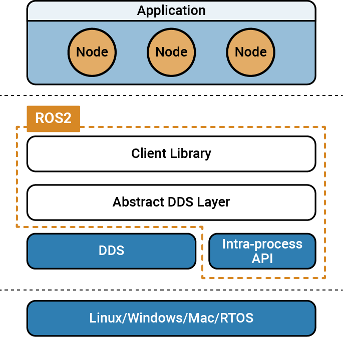
\includegraphics[width=0.6\textwidth]{img/software/ros_middleware_overview_mathworks.png}
    \caption{ROS 2 Middleware Overview: Integration of DDS in ROS 2}
    \label{fig:ros2_middleware}
\end{figure}


\subsubsection{Nodes, Topics, Services, and Actions}
ROS 2 uses a modular architecture composed of nodes, each encapsulating specific functionalities such as sensor processing, localization, and control \cite{doi:10.48550/arXiv.2305.09933}. Nodes interact exclusively through clearly defined interfaces:
\begin{itemize}
    \item Topics: Provide asynchronous data communication channels ideal for continuous sensor data streams, such as LiDAR point clouds and odometry updates.
    \item Services: Enable synchronous request-response communication, useful for discrete commands or status checks like initiating sensor calibration.
    \item Actions: Support goal-oriented asynchronous tasks with feedback loops, beneficial for complex operations such as navigation or docking maneuvers.
\end{itemize}

\begin{figure}[h]
    \centering
    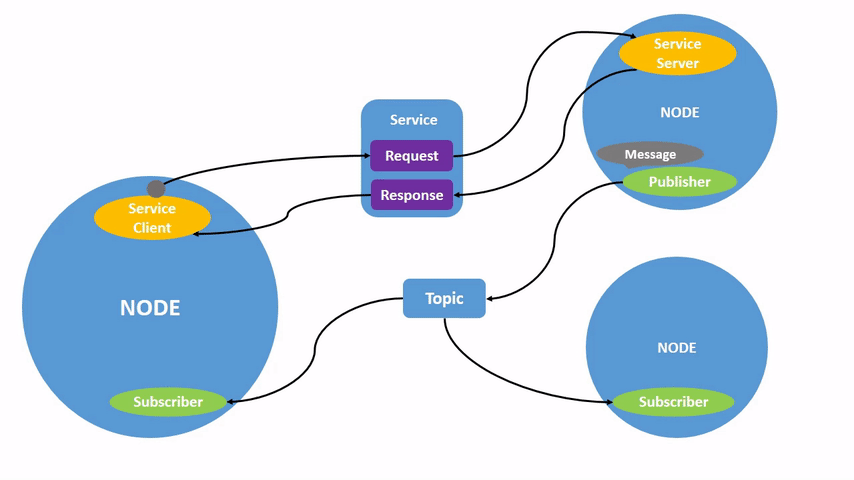
\includegraphics[width=0.7\textwidth]{img/software/node_topic_service_ros2doc.png}
    \caption{ROS 2 Nodes, Topics, Services, and Actions}
    \label{fig:ros2_comm_model}
\end{figure}

\subsubsection{ROS 2 Tooling and Development Workflow}
ROS 2 provides comprehensive tooling to streamline software development, deployment, and debugging. The colcon build tool efficiently manages workspace compilation and dependency resolution. The ros2 launch system simplifies system initialization, configuration, and node orchestration. Diagnostic and visualization tools, including RViz2 and RQT, support real-time monitoring, debugging, and system introspection, essential for verifying proper integration and functionality during development.

\subsection{Simultaneous Localization and Mapping (SLAM)}
\subsubsection{Overview and Importance}
Simultaneous Localization and Mapping (SLAM) is a fundamental technique in autonomous robotics, enabling a robot to concurrently build a map of an unknown environment and estimate its position within that map. SLAM addresses the critical challenge of operating autonomously in GPS-denied or dynamically changing areas, making real-time navigation decisions without prior environmental knowledge. 2D SLAM is commonly selected in many robotic applications due to its computational efficiency, suitability for real-time execution on resource-constrained hardware, and compatibility with planar LiDAR sensors.


\subsubsection{Implementation Using SLAM Toolbox}
The ROS 2 SLAM Toolbox package is utilized to achieve robust 2D SLAM capabilities \cite{Macenski2021}. SLAM Toolbox offers efficient real-time pose-graph SLAM functionality tailored specifically for ROS 2 Humble, including incremental and lifelong mapping, loop closure detection, and pose graph optimization. This toolbox was selected due to its active development, seamless integration with ROS 2, and proven real-world performance. Alternative approaches, such as Google Cartographer and GMapping, were considered but not pursued due to reduced support and incomplete ROS 2 compatibility.

\subsubsection{Pose Graph Mapping, Real-Time Updates, and Loop Closure}

SLAM Toolbox applies a pose-graph approach, incrementally constructing an occupancy grid map by aligning new LiDAR scans with previous ones using scan matching algorithms such as Iterative Closest Point (ICP). Each aligned scan contributes constraints to the pose graph, continuously improving localization accuracy as the robot navigates.

To support real-time performance, parameters such as scan insertion frequency, resolution, and search algorithms are optimized for resource-constrained hardware like the Raspberry Pi. The map updates dynamically with new observations, enabling immediate navigation in previously unmapped areas.

Over time, localization drift may accumulate. To address this, SLAM Toolbox performs loop closure detection by recognizing revisited areas and matching current scans with historical data. Upon detecting a loop closure, additional constraints are added to the pose graph, triggering a global optimization step using solvers like Google\textquotesingle s Ceres Solver. This process corrects accumulated drift and improves overall map consistency. SLAM Toolbox\textquotesingle s lifelong mapping feature enables continuous refinement and optimization, increasing long-term reliability in dynamic environments.


\begin{figure}[h]
    \centering
    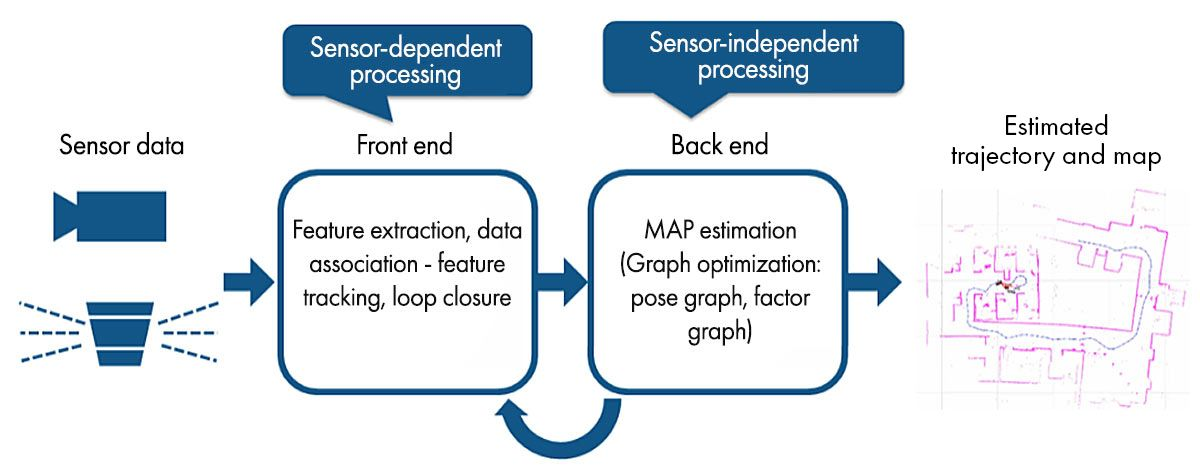
\includegraphics[width=0.8\textwidth]{img/software/slam_pose_graph.jpg}
    \caption{Pose-Graph SLAM: Front-End Feature Extraction and Back-End Optimization}
    \label{fig:slam_pose_graph}
\end{figure}

\subsection{Navigation and Path Planning}
\subsubsection{Overview of the ROS 2 Navigation Stack}
The ROS 2 Navigation Stack (Nav2) provides a robust, modular, and widely-adopted framework essential for autonomous navigation tasks. It integrates localization, global and local planning, obstacle avoidance, and recovery strategies into a cohesive architecture. Utilizing a behavior tree approach, Nav2 orchestrates these functionalities dynamically, offering flexibility and adaptability crucial for real-world autonomous vehicle operations\cite{MACENSKI2023104493}.

\subsubsection{Localization from SLAM in ROS 2 Navigation Stack}
The SLAM-generated occupancy grid map and localization data are directly integrated into the ROS 2 Navigation Stack (Nav2). SLAM Toolbox continuously updates the `map->odom` transform, providing real-time localization of the vehicle within the constructed map. 

This transform enables Nav2\textquotesingle s core components, including the global planner (`planner\_server`) and local controller (`controller\_server`), to operate with precise localization input. The AMCL (Adaptive Monte Carlo Localization) node, when used with an existing static map, further refines localization accuracy by processing sensor (`/scan`) data. 

Nav2 leverages this accurate localization to:

\begin{itemize}
    \item Perform global and local path planning based on updated map information.
    \item Execute obstacle avoidance using costmaps (\texttt{global\_costmap}, \texttt{local\_costmap}).
    \item Enable smooth motion control via \texttt{cmd\_vel} commands sent to the base controller.
\end{itemize}

Ensuring synchronization between SLAM and Nav2 is critical for reliable autonomous navigation. The bt\_navigator component in Nav2 orchestrates navigation actions (`NavigateToPose`, `FollowPath`), ensuring seamless integration between localization, planning, and control. 

\begin{figure}[h]
    \centering
    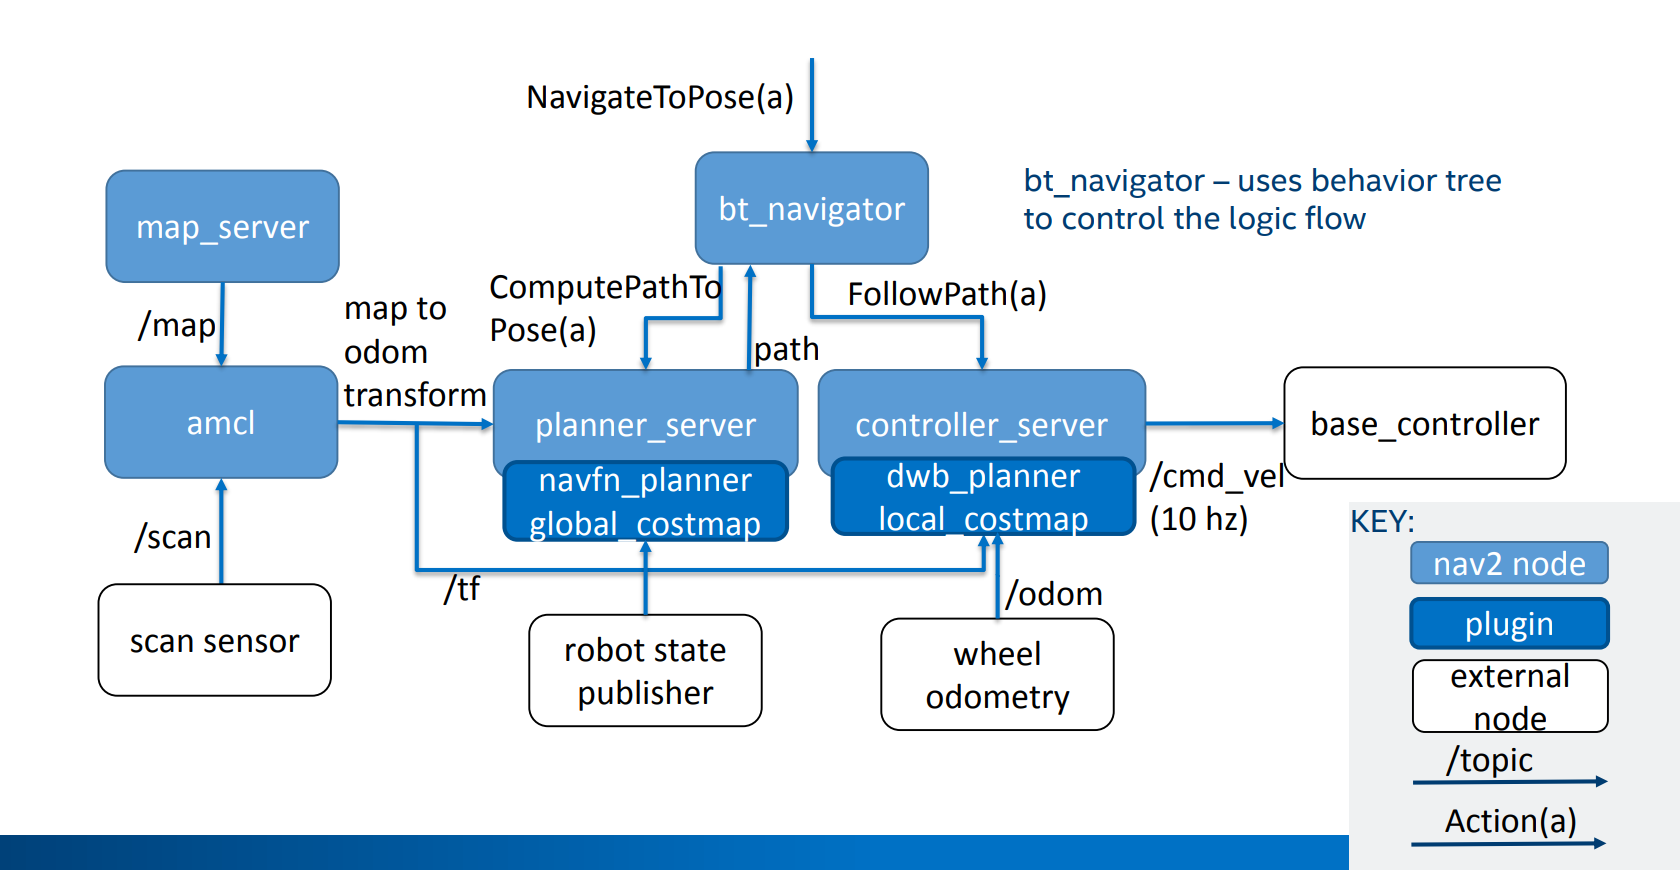
\includegraphics[width=0.9\textwidth]{img/software/nav2_architecture.png}
    \caption{ROS 2 Navigation Stack (Nav2) Architecture: Integration of Localization, Planning, and Control}
    \label{fig:nav2_architecture}
\end{figure}

\subsubsection{Global and Local Planning Overview}

In the ROS 2 Navigation Stack (Nav2), global planners compute high-level paths from the robot\textquotesingle s current location to a specified goal using occupancy grid maps. Local planners are responsible for generating real-time velocity commands that enable the robot to follow the planned path while dynamically avoiding obstacles. Nav2 supports a variety of planning algorithms for both global and local planning tasks. Examples include A\* and Dijkstra for global path computation, and DWB (Dynamic Window Approach) or TEB (Timed Elastic Band) for local trajectory optimization. The choice of planners can be tailored to the robot\textquotesingle s kinematic model, environmental complexity, and desired navigation behavior.



\subsubsection{Costmaps and Obstacle Avoidance}
Costmaps serve as the underlying representation of the navigational environment, encoding static and dynamic obstacles in a layered grid structure. Nav2 employs three primary costmap layers:
\begin{itemize}
    \item Static Layer
    \begin{itemize}
        \item Represents fixed obstacles derived from pre-built or SLAM-generated maps.
    \end{itemize}

    \item Obstacle Layer
    \begin{itemize}
        \item Continuously updated in real-time with sensor data, capturing moving or unforeseen obstacles.
    \end{itemize}

    \item Inflation Layer
    \begin{itemize}
        \item Provides safety margins around obstacles by inflating obstacle regions to ensure safe distances and smoother trajectory generation.
    \end{itemize}
\end{itemize}

\subsubsection{Dynamic Replanning and Recovery Strategies}

Real-world autonomous navigation necessitates robust strategies to handle unforeseen environmental changes or navigational failures.

\begin{itemize}
    \item \textbf{Dynamic Replanning}:  Nav2 regularly updates the global path to adapt to new obstacles or environmental changes, typically on the order of seconds. This ensures the vehicle can continuously adjust its path in response to dynamic conditions without human intervention.
    
    \item \textbf{Recovery Behaviors}: Nav2 incorporates predefined recovery mechanisms activated through behavior trees when encountering navigational difficulties. Common recovery behaviors include:
    \begin{itemize}
        \item \textbf{Spin Recovery}: Rotating the vehicle in place to scan surroundings and update the local environment representation.
        \item \textbf{Clearing Costmap}: Resetting local or global costmaps to remove outdated obstacle data.
        \item \textbf{Backup and Rotate Maneuvers}: Allowing the vehicle to reposition itself when facing persistent obstacles.
    \end{itemize}
\end{itemize}



\subsection{Control Systems}
\subsubsection{Motor Control Fundamentals}
Motor control is a critical component of autonomous robotic systems, involving precise regulation of actuator movements to achieve desired trajectories. Effective motor control often requires real-time adjustments to account for environmental factors, actuator dynamics, and external disturbances. Closed-loop control methods, incorporating sensor feedback, are typically employed in robotic systems to ensure accurate and stable actuator performance.
\subsubsection{ROS 2 Control Framework (ros2\_control)}
The ros2\_control framework provides a modular and standardized approach to managing robotic actuators within the ROS 2 ecosystem. It enables efficient hardware abstraction, controller management, and real-time actuator control while ensuring safe and scalable system operation.

At its core, ros2\_control consists of:
\begin{itemize}
    \item Controllers: Independent modules that regulate actuators based on input commands and sensor feedback. Multiple controllers can be managed dynamically to support various motion control strategies.
    \item Controller Manager: A centralized entity responsible for dynamically loading, unloading, and supervising controllers, ensuring seamless system operation.
    \item Hardware Interfaces: These provide communication between controllers and physical components. Interfaces are typically categorized into:
    \begin{itemize}
        \item State Interfaces: Read-only interfaces that relay sensor data and system feedback.
        \item Command Interfaces: Read-write interfaces allowing controllers to send actuation commands to motors or other robotic components.
    \end{itemize}
    \item Hardware Resources: The physical components, such as sensors, actuators, and transmission mechanisms, that interact with the control system.
\end{itemize}

A key advantage of ros2\_control is its flexibility and scalability. It enables robots to seamlessly switch between different controllers, optimize resource allocation, and support real-time operation across diverse robotic platforms. The framework is widely adopted in differential drive robots, robotic arms, and mobile platforms, providing an efficient and structured approach to motion control.

\begin{figure}[H]
    \centering
    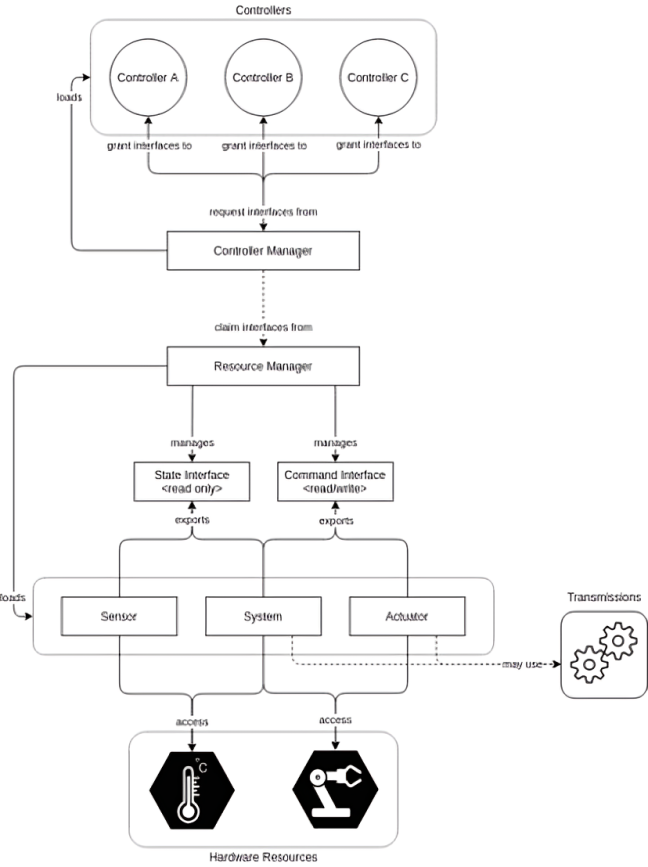
\includegraphics[width=0.7\textwidth, height=0.7\textheight, keepaspectratio]{img/software/ros2_control_architecture.png}
    \caption{ROS 2 Control Framework: Controller Manager, Resource Manager, and Hardware Interfaces}
    \label{fig:ros2_control_architecture}
\end{figure}



\subsubsection{PID Controllers: Fundamentals and Tuning}
Proportional-Integral-Derivative (PID) controllers are widely utilized in robotic applications for motion control due to their simplicity, robustness, and proven effectiveness. A PID controller adjusts actuator commands based on the difference between desired and measured states, continuously minimizing errors in real time. Proper tuning of PID gains (proportional, integral, derivative) is essential to avoid instability or sluggish system response, typically achieved through iterative adjustment informed by experimental observations or established tuning methodologies.
\subsubsection{Motion Control Algorithms}
Motion control algorithms translate navigation commands into actionable actuator signals. Two common algorithms for mobile robots are:
\begin{itemize}
    \item Differential Drive Control
    \begin{itemize}
        \item Frequently used in robotic platforms with independently driven wheels, differential drive achieves steering by adjusting relative wheel speeds. This allows precise maneuverability, including zero-radius turns, making it highly suitable for compact, indoor robotic systems.
    \end{itemize}


    \item Ackermann Steering Control
    \begin{itemize}
        \item Widely adopted for car-like vehicles, Ackermann steering provides smooth turning behavior by controlling wheel angles and velocity. Path-tracking algorithms such as Pure Pursuit and Stanley controllers are commonly employed to follow defined trajectories accurately and stably, particularly beneficial for higher-speed, outdoor autonomous vehicles.
    \end{itemize}
\end{itemize}

\subsection{Visualization}
Visualization tools are essential components in robotic software development, enabling developers to monitor real-time system behavior, diagnose problems rapidly, and interact with complex robotic systems intuitively. Within the ROS 2 ecosystem, the visualization and graphical monitoring of data streams and system states are primarily handled through tools such as RViz and RQT.
\subsubsection{Robot Visualization with RViz}
RViz (ROS Visualization) is a sophisticated 3D visualization software package specifically designed for use with ROS-based robotic systems. It provides real-time graphical representations of sensor data, robot configurations, and state information, facilitating both development and debugging processes. In autonomous robotics applications, especially those involving complex sensor fusion and navigation tasks, visualizing the data is critical for verifying system performance and identifying anomalies.

RViz supports a wide range of visualization types, including point clouds, coordinate frames, occupancy maps, robot models, and planned paths. Its interactive and modular interface helps developers gain real-time insights into system behavior and detect issues quickly.

\subsubsection{System Monitoring and Control with RQT}
RQT (ROS Qt Toolkit) is a versatile graphical user interface framework built on top of Qt, offering a flexible environment for system monitoring, debugging, and basic robot control within ROS systems. Its modular architecture allows developers to customize the user interface by selecting from numerous available plugins or creating custom plugins as needed.

RQT includes plugins for real-time topic plotting, node management, parameter tuning, and basic teleoperation. These features make it a valuable tool during development and testing phases by offering immediate system insights and interaction capabilities.

The combination of visualization, interaction, and real-time monitoring offered by RQT accelerates the software development cycle by providing immediate insights into system operation and performance. It complements RViz by handling numerical and textual data, offering developers a comprehensive suite for effective system debugging and iterative refinement.

\subsection{Simulation and Testing}
Simulation plays a crucial role in the development, verification, and validation of autonomous vehicle software, enabling safe, efficient, and repeatable testing of robotic algorithms in virtual environments. This section outlines the simulation environment and methods utilized in the project, including robot model definition, sensor data simulation, algorithm validation, and debugging strategies.
\subsubsection{Gazebo Simulation Environment}

Gazebo is a widely used robotic simulation environment that integrates seamlessly with ROS 2, enabling virtual testing and development of robotic systems. It supports simulation of robot dynamics, sensor data, and environmental interactions, allowing developers to evaluate SLAM, navigation, perception, and control algorithms in a safe and repeatable manner.

By replicating real-world conditions virtually, Gazebo helps identify issues early in the development cycle, reducing the risk of hardware damage and improving overall system reliability. It plays a key role in accelerating development and debugging processes by enabling rapid prototyping and validation without requiring physical deployment.

\subsubsection{Robot Model Definition (URDF and Xacro)}
Accurate simulation requires a realistic representation of the robot\textquotesingle s physical characteristics and sensor layout. The robot was defined using the Unified Robot Description Format (URDF), an XML-based description standard widely adopted within ROS. URDF captures essential physical properties, including kinematic structure, inertial parameters, and sensor placements. To simplify model management, URDF files were generated and managed using Xacro, an XML macro language that provides modularity and reusability through parameters and macros. The structured robot model serves as the foundation for simulations, accurately reflecting hardware constraints, sensor perspectives, and physical interactions within Gazebo. This ensures simulation fidelity and enables meaningful insights into robot performance under various test conditions.
\subsubsection{Sensor Simulation and Data Validation}
An essential advantage of simulation-based testing is the ability to simulate sensor data streams closely resembling real-world conditions. Gazebo supports realistic simulation of sensors such as LiDAR, IMU, camera modules, and wheel encoders. Sensor simulation incorporates noise and error models to replicate real-world inaccuracies, enabling validation of sensor data processing algorithms and sensor fusion techniques used in localization, mapping, and navigation. By conducting sensor validation in simulation, issues like improper data synchronization, sensor misalignments, and data processing errors are identified and addressed early, improving reliability before hardware integration.
\subsection{Multi-Machine Communication}

Reliable communication between multiple computational devices is essential in autonomous robotic systems, especially when processing tasks are distributed across onboard and external computing units. ROS 2 provides native support for distributed systems through its middleware layer, allowing seamless data exchange across machines.

This capability enables developers to offload computationally intensive tasks, such as visualization, logging, or high-level planning, to more powerful machines, while real-time tasks like sensor data processing and actuator control remain on embedded platforms. ROS 2's decentralized, peer-to-peer communication model, based on the Data Distribution Service (DDS), ensures robust and scalable multi-machine deployments without relying on a central server.
\subsubsection{ROS 2 Networking for Distributed Computation}
ROS 2 inherently supports distributed computing through its use of the Data Distribution Service (DDS) middleware, enabling decentralized, peer-to-peer communication across networked computers. DDS allows nodes running on separate machines to transparently exchange data, simplifying the deployment of computationally demanding tasks such as visualization, logging, and high-level planning on powerful desktop machines, while delegating real-time sensor processing and actuator control to the onboard system (e.g., Raspberry Pi). The decentralized DDS architecture eliminates the single point of failure present in earlier ROS versions, making multi-machine deployments robust, scalable, and fault-tolerant.


\subsubsection{Time Synchronization and Data Consistency}

Accurate time synchronization between distributed computers is essential for ensuring data consistency, sensor fusion accuracy, and precise localization and navigation tasks. ROS~2 relies on synchronized system clocks (e.g., using the Network Time Protocol~(NTP) or the Precision Time Protocol~(PTP)) across machines to correctly timestamp sensor data and maintain a consistent interpretation of temporal relationships. 

Proper synchronization mitigates issues such as latency-induced localization drift or sensor misalignment, thereby improving the reliability and accuracy of distributed data fusion processes. Standard practices involve configuring NTP or PTP on all involved machines, ensuring high-quality data exchange and robust system operation.
\end{document}
\newpage
\documentclass[english,project]{buwthesis}
\begin{document}
\section{Hardware Overview}



\subsection{Car}
\begin{itemize}
    
    \item Product Dimension: 106 x 62 x 46 cm; 14 kg
    \item 2 x 25-watt motor (total 50 watts), quiet tyres with a soft rubber ring.
    \item 2.4 GHz remote control, seat belt, horn.
    \item 12 Volt 4,5 Ah battery, up to 6 km/h speed
\end{itemize}

\begin{figure}[ht]
    \centering
    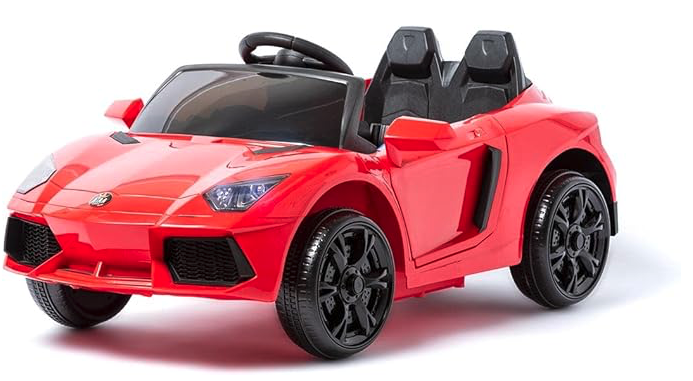
\includegraphics[width=0.6\textwidth]{img/car.png}
    \caption{Car}
    \label{fig:car}
\end{figure}


\subsection{Raspberry Pi 4 Model B}


Raspberry Pi 4 Model B features a high-performance 64-bit quad-core processor,
dual-display support at resolutions up to 4K via a pair of micro HDMI ports, hardware
video decode at up to 4Kp60, up to 8GB of RAM, dual-band 2.4/5.0 GHz wireless LAN,
Bluetooth 5.0, Gigabit Ethernet, USB 3.0, and PoE capability (via a separate PoE HAT
add-on). For the end user, Raspberry Pi 4 Model B provides desktop performance
comparable to entry-level x86 PC systems.\cite{raspberrypi4productbrief}

\textbf{Specifications:}
\begin{itemize}
    \item Processor: Broadcom BCM2711, quad-core Cortex-A72 (ARM v8) 64-bit SoC @ 1.5GHz
    \item Memory: 4GB  LPDDR4-3200 SDRAM with on-die ECC
    \item Connectivity: 2.4 GHz and 5.0 GHz IEEE 802.11b/g/n/ac wireless LAN, Bluetooth 5.0, BLE
    \item Input power: 5V DC via USB-C connector (minimum 3A)
\end{itemize}

*This product should only be connected to an external power supply rated at 5V/3A DC or 5.1V/ 3A DC minimum.

\begin{figure}[ht]
    \centering
    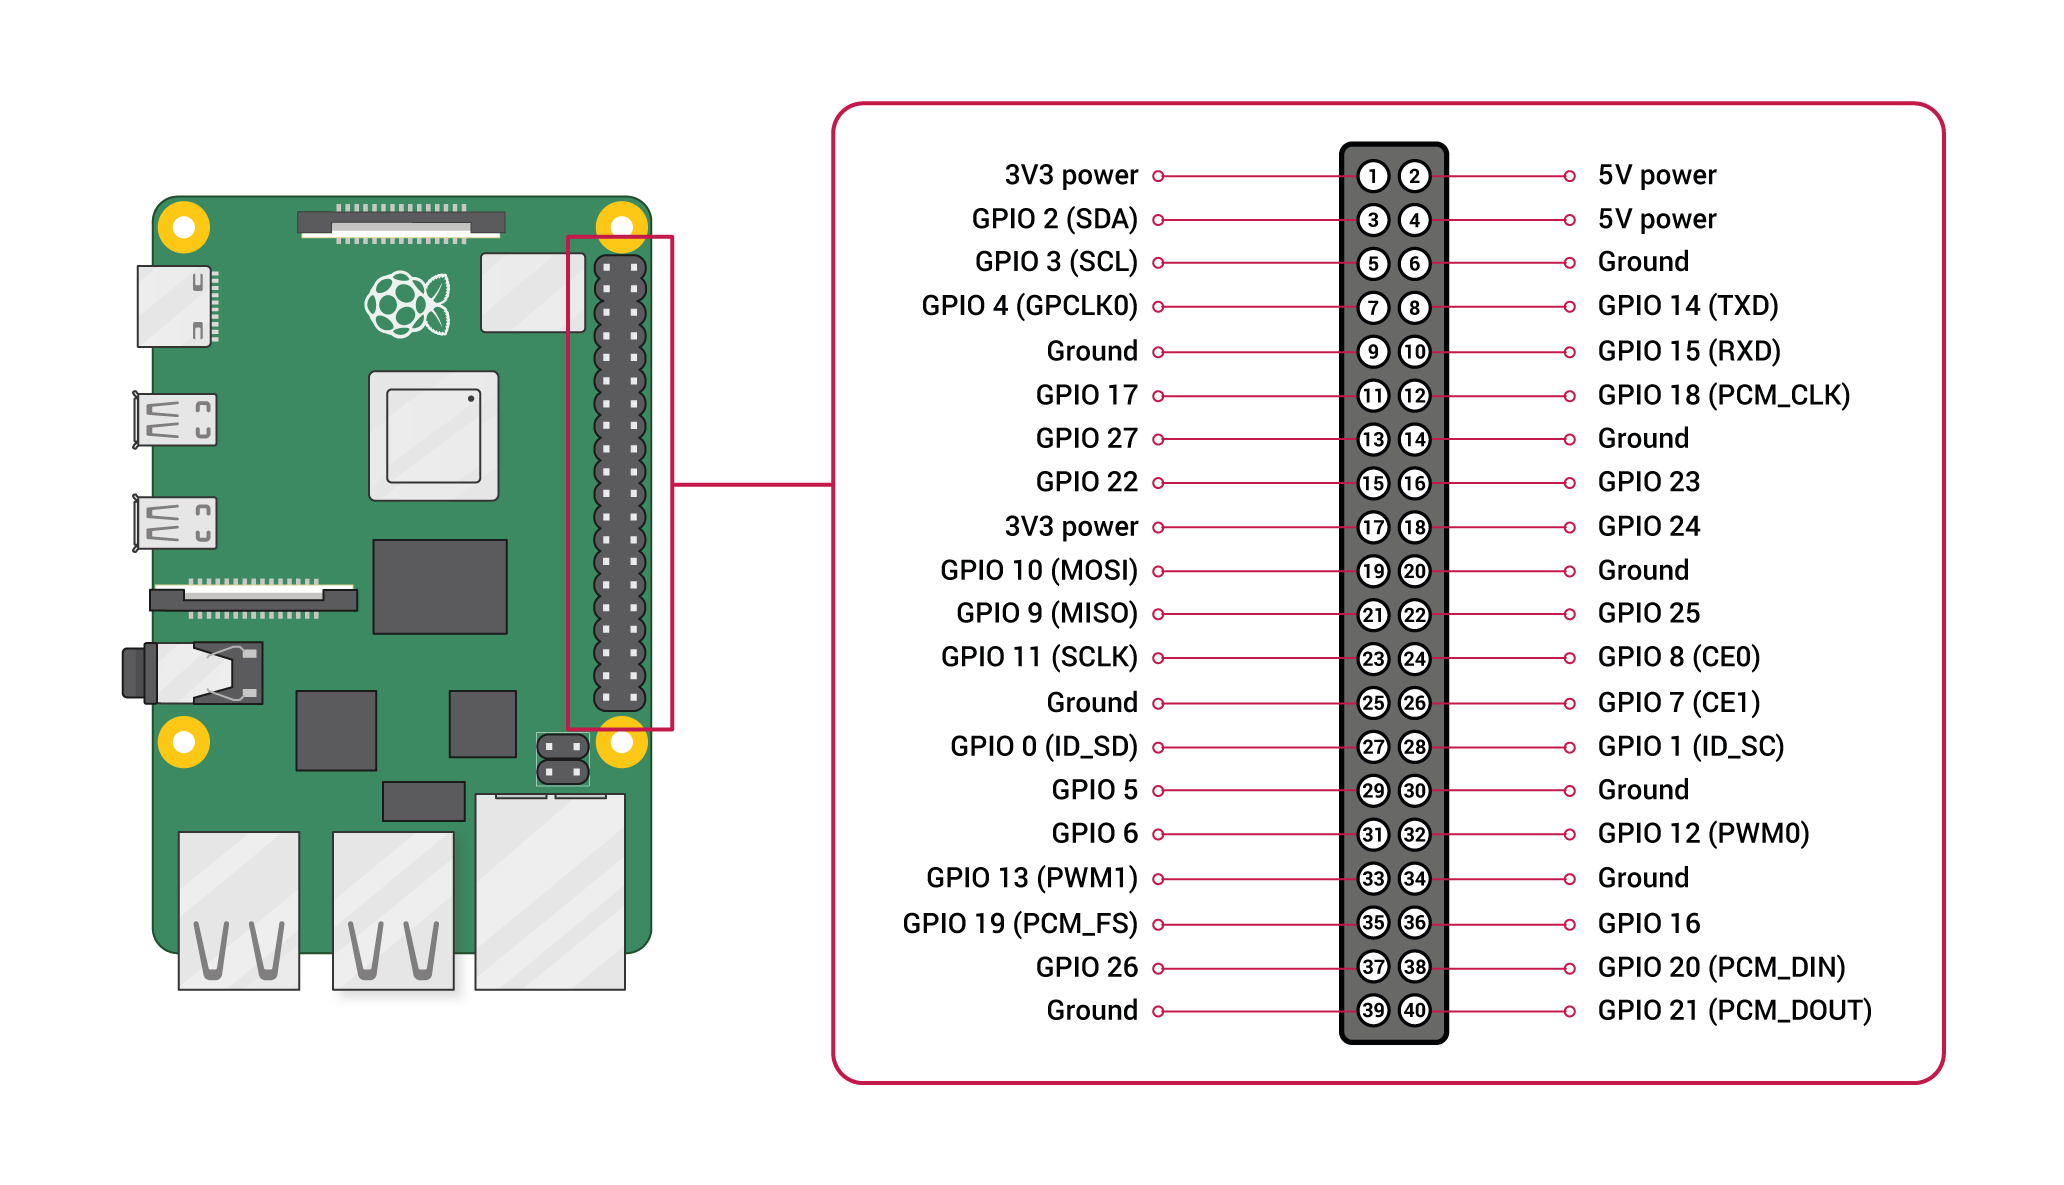
\includegraphics[width=0.8\textwidth]{img/raspberrypiblock.png}
    \caption{Raspberry Pi 4 Block Diagram\cite{raspberrypi4productbrief}}
    \label{fig:raspberrypiblock}
\end{figure}


\subsection{Arduino Nano}

Arduino Nano is an intelligent development board designed for building faster prototypes with the smallest dimension. Arduino Nano being the oldest member of the Nano family, provides enough interfaces for your breadboard-friendly applications. At the heart of the board is ATmega328 microcontroller clocked at a frequency of 16 MHz featuring more or less the same functionalities as the Arduino Duemilanove. The board offers 20 digital input/output pins, 8 analog pins, and a mini USB port. \cite{arduinoNanoDatasheet}

\textbf{Specifications:}
\begin{itemize}
    \item Microcontroller: ATmega328 16 MHz, 2KB SRAM, 32KB Flash, 1KB EEPROM
    \item Input power: 5V DC via Mini-B USB
    \item Pins:
    \begin{itemize}
        \item Built-in LED Pin:13
        \item Digital I/O Pins:14
        \item Analog input pins:8
        \item PWM pins:6
    \end{itemize}

\end{itemize}

\begin{figure}[ht]
    \centering
    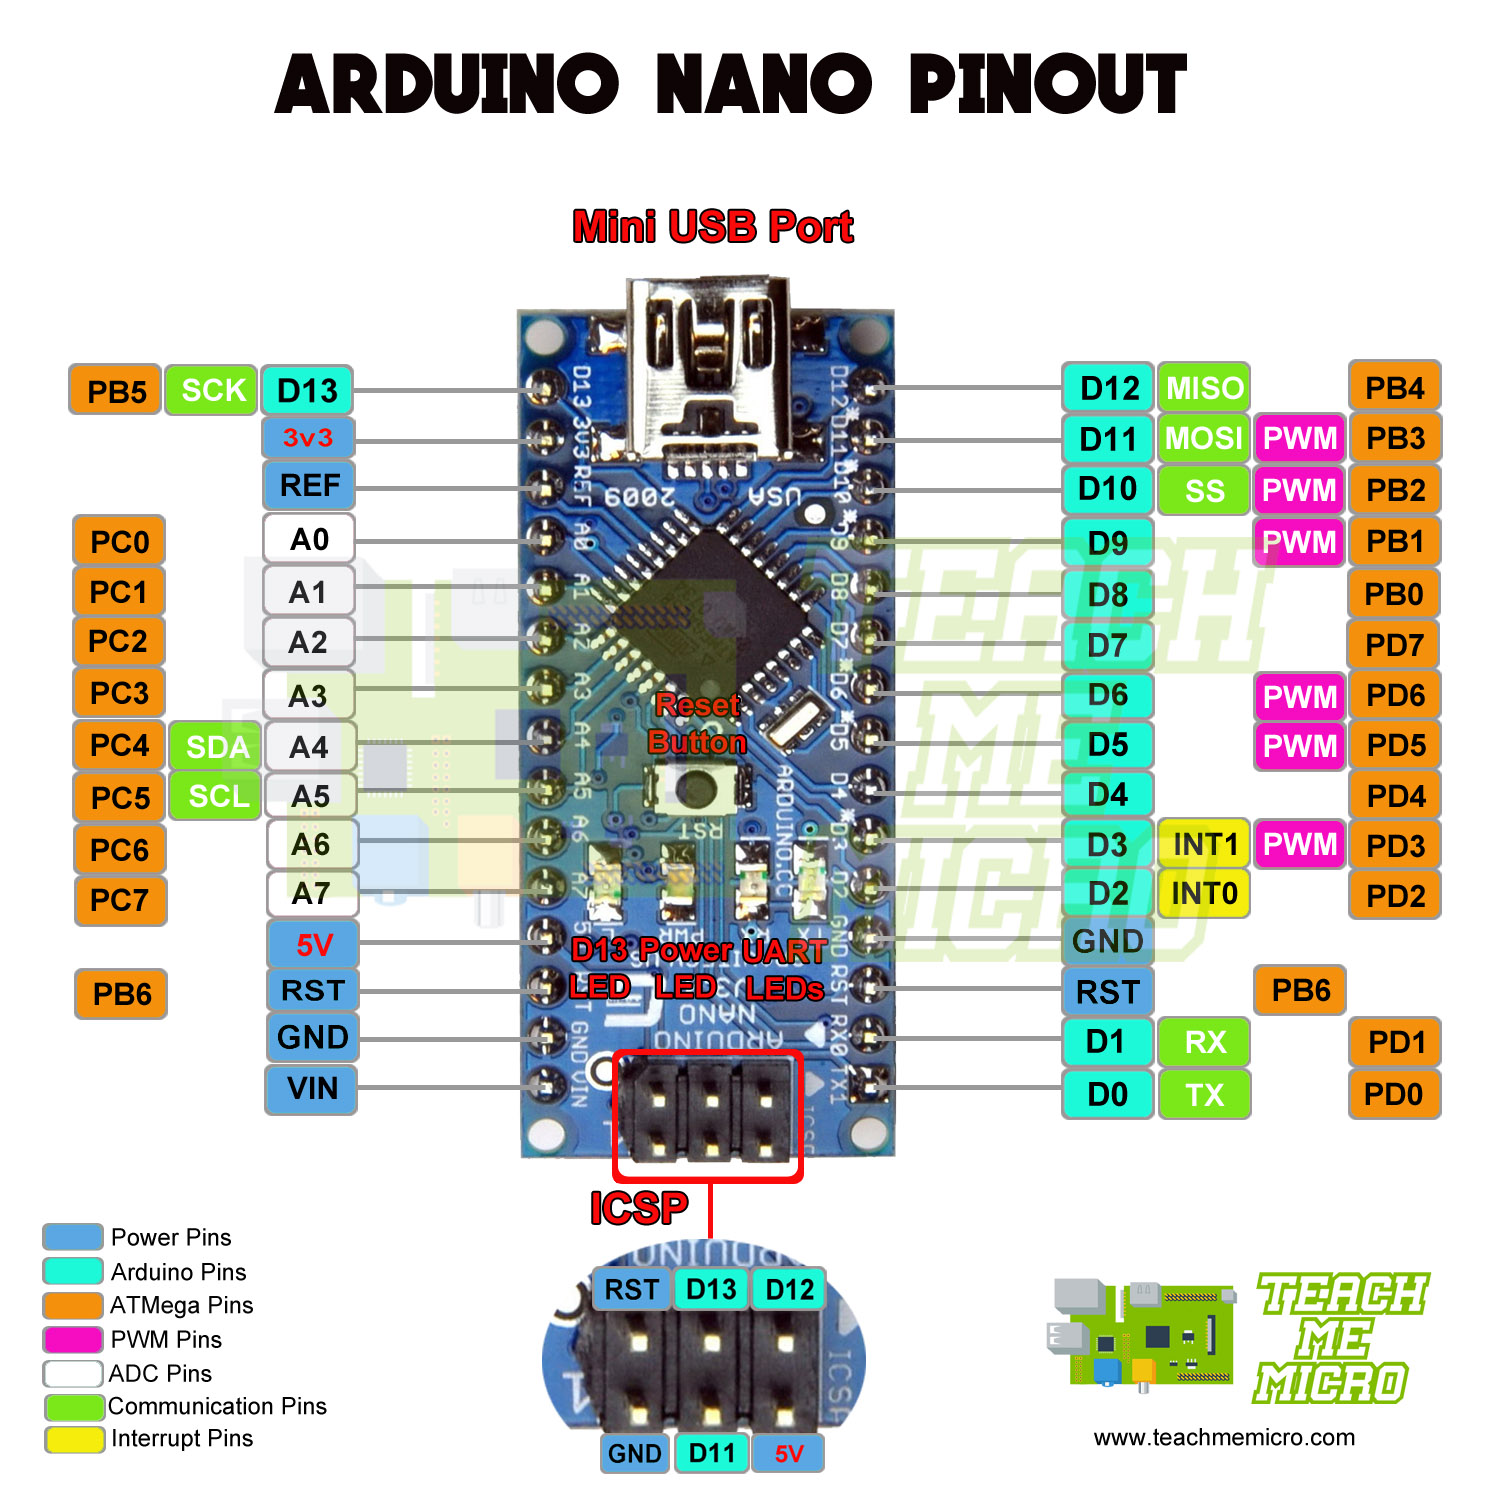
\includegraphics[width=0.6\textwidth]{img/arduinonanoblock.png}
    \caption{Arduino Nano Block Diagram\cite{arduinoNanoDatasheet}}
    \label{fig:arduinonanoblock}
\end{figure}



\subsection{Rplidar A1}

RPLIDAR A1 is a low cost 360 degree 2D laser scanner (LIDAR) solution developed by SLAMTEC. The system can perform 360 degree scan within 12 meter range. The produced 2D point cloud data can be used in mapping, localization and object/environment modeling. RPLIDAR A1's scanning frequency reached 5.5hz when sampling 1450 points each round. And it can be configured up to 10hz maximum.\cite{rplidarA1M8Datasheet}

\begin{table}[ht]
\centering
\begin{tabular}{|l|c|p{9cm}|}\hline
Distance         & mm       & Current measured distance value between the rotating core of the RPLIDAR A1 and the sampling point. \\ \hline
Heading          & degree   & Current heading angle of the measurement. \\ \hline
Quality          & level    & Quality of the measurement. \\ \hline
Start Flag       & (Boolean) & Flag of a new scan. \\ \hline
\end{tabular}
\caption{The RPLIDAR A1 Sample Point Data Information\cite{rplidarA1M8Datasheet}}
\label{tab:rplidar_data_info}
\end{table}


\subsection{Color Sensor - TCS 34725}

The TCS3472 device provides a digital return of red, green, blue (RGB), and clear light sensing values. An IR blocking filter, integrated on-chip and localized to the color sensing photodiodes, minimizes the IR spectral component of the incoming light and allows color measurements to be made accurately. The high sensitivity, wide dynamic range, and IR blocking filter make the TCS3472 an ideal color sensor solution for use under varying lighting conditions and through attenuating materials.\cite{tcs34725datasheet}

\textbf{Features:}
\begin{itemize}

    \item Red, Green, Blue (RGB), and Clear Light Sensing with IR Blocking Filter
    \begin{itemize}
        \item Programmable Analog Gain and Integration Time
        \item 3,800,000:1 Dynamic Range
        \item Very High Sensitivity - Ideally Suited for operation Behind Dark Glass
    \end{itemize}

    \item Maskable Interrupt
    \begin{itemize}
        \item Programmable Upper and Lower Thresholds with Persistence Filter
    \end{itemize}
    
    \item Power Management
    \begin{itemize}
        \item Low Power - 2.5-mA Sleep State
        \item 65-mA Wait State with Programmable Wait State Time from 2.4 ms to > 7 Seconds
    \end{itemize}
    
    \item I2C Fast Mode Compatible Interface
    \begin{itemize}
        \item Data Rates up to 400 kbit/s
        \item Input Voltage Levels Compatible with VDD or 1.8 V Bus
    \end{itemize}
    
    \item Register Set and Pin Compatible with the TCS3x71 Series
    
    \item Small 2 mm y 2.4 mm Dual Flat No-Lead (FN) Package

\end{itemize}


\begin{figure}[ht]
    \centering
    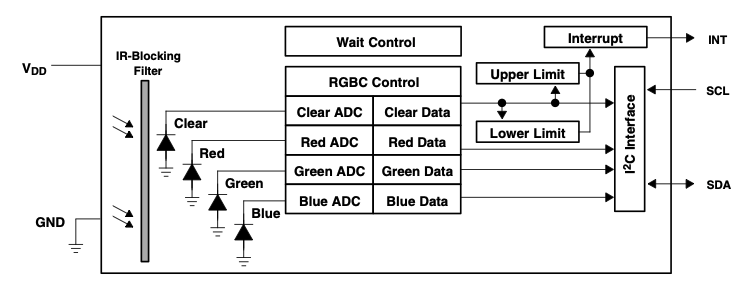
\includegraphics[width=0.8\textwidth]{img/colorsensorblockdiagram.png}
    \caption{Color Sensor TCS 34725 Terminal Block Diagram\cite{tcs34725datasheet}}
    \label{fig:colorsensorblockdiagram}
\end{figure}


\begin{table}[ht]
\centering
\begin{tabular}{|c|c|l|}
\hline
\textbf{Terminal Name} & \textbf{No.} & \textbf{Description} \\ \hline
GND                   & 3            & Power supply ground. All voltages are referenced to GND. \\ \hline
INT                   & 5            & Interrupt - open drain (active low). \\ \hline
NC                    & 4            & No connect - do not connect. \\ \hline
SCL                   & 2            & I\textsuperscript{2}C serial clock input terminal - clock signal for I\textsuperscript{2}C serial data. \\ \hline
SDA                   & 6            & I\textsuperscript{2}C serial data I/O terminal - serial data I/O for I\textsuperscript{2}C. \\ \hline
$V_{DD}$              & 1            & Supply voltage. \\ \hline
\end{tabular}
\caption{Color Sensor TCS 34725 Terminal Functions\cite{tcs34725datasheet}}
\label{tab:colorsensorterminalfunction}
\end{table}


\subsection{Motor Driver - ZK BM1}

ZK-BM1 10A 3-18V DC PWM Dual Motor Driver. 3-18VDC can control 2 motors independently. Single channel operating current is 10 amps. Since the current is above 8 amperes, it is recommended to increase the heat dissipation. The motor driver can move the motor forward and backward and adjust its speed. \cite{motorobitZKBM1}

\textbf{Things to Consider During Use:}
\begin{itemize}
    \item When changing the forward-backward direction of the motor, be sure to stop the motor and change direction
    \item Make connections carefully, there is no reverse polarity protection
    \item PWM control frequency should not exceed 2kHz. Otherwise, the module will be damaged
    \item If the Operating Current exceeds 8 amperes, heat dissipation equipment must be added
\end{itemize}

\textbf{Specifications:}
\begin{itemize}
    \item Supply Voltage: 3-18V DC
    \item Operating Current: 10 A for each channel
    \item Supported PWM Frequency Range: 0 - 2 kHz
    \item Operating Temperature Range: -25 ~ 85C
    \item Module Size: 49x39x14mm
\end{itemize}

\begin{figure}[ht]
    \centering
    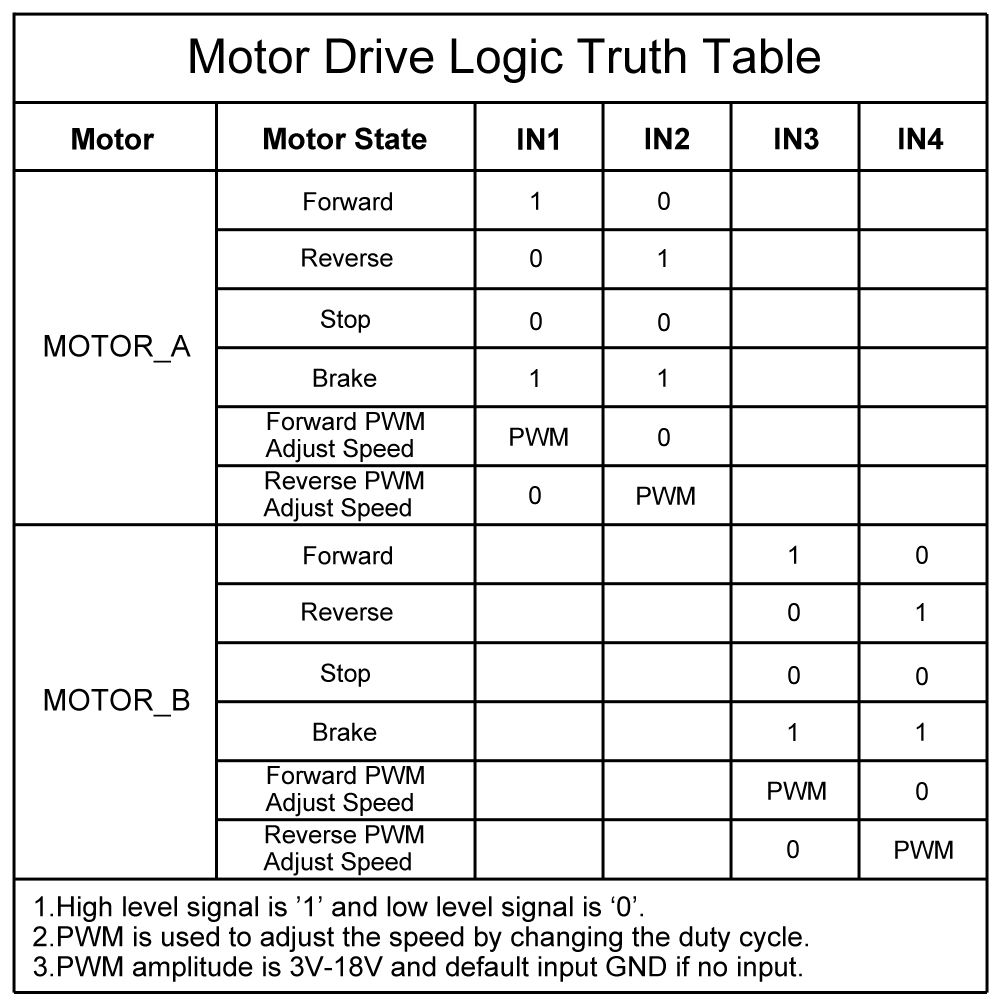
\includegraphics[width=0.4\textwidth]{img/motordriverlogic.png}
    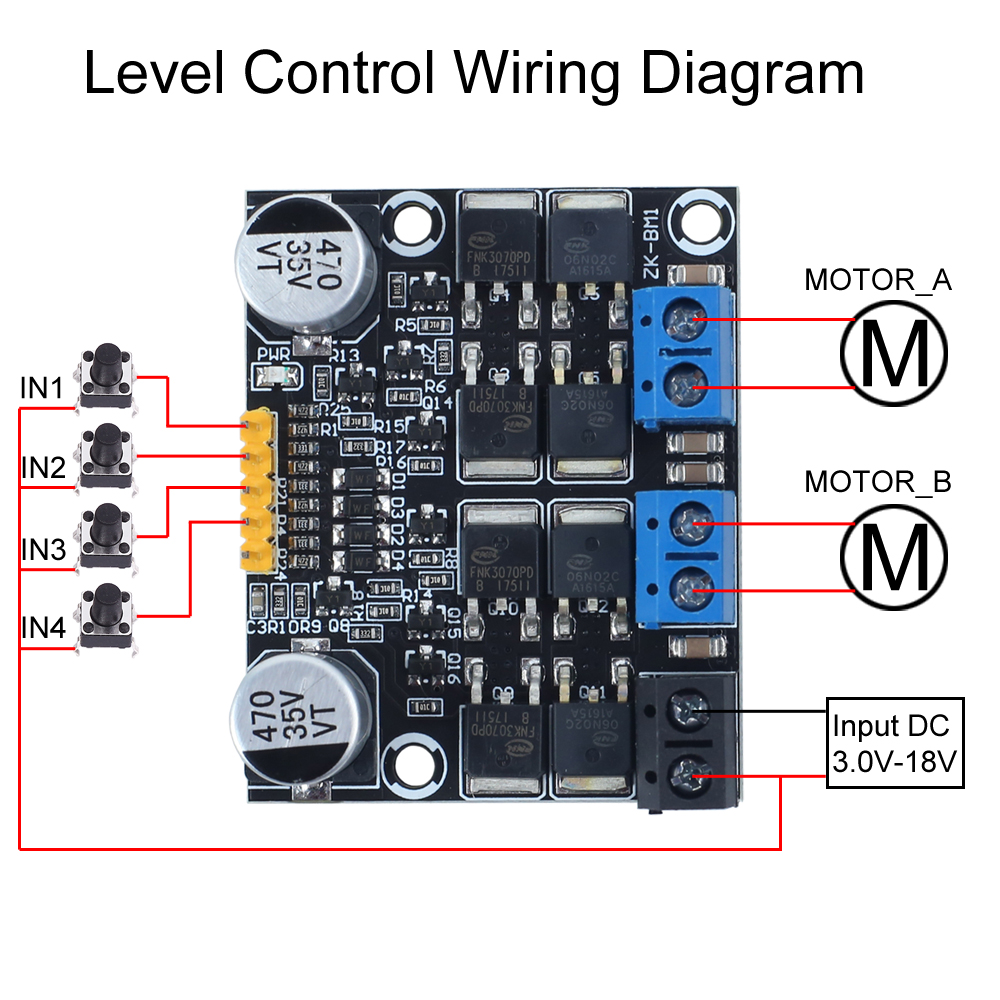
\includegraphics[width=0.4\textwidth]{img/motordriverwiring.png}
    \caption{Motor Driver Logic Table and Wiring Digram\cite{motorobitZKBM1}}
    \label{fig:motordriverlogic}
\end{figure}

\subsection{IMU Sensor - GY 521}

The GY-521 is a module based on MPU6050 sensor chip which is a system that combines a 3-axis gyroscope, a 3-axis accelerometer and a digital thermometer. Its special feature is the built-in hardware DMP (Digital Motion Processor) unit, which facilitates the conversion of processed data from all three sensors to a specific position relative to the Earth, thus relieving the microcontroller. The DMP unit can be programmed to also use an external magnetometer for its calculations.\cite{mpu6050datasheet}

\textbf{Features:}
\begin{itemize}

    \item \textbf{Gyroscope Features:}
    \begin{itemize}
        \item Digital output X, Y, and Z-Axis angular rate sensors (gyroscopes) with a user-programmable full-scale range of \[\pm 250,\ \pm 500,\ \pm 1000,\ \text{and}\ \pm 2000\ \text{/sec}\]
        \item Integrated 16-bit ADCs enable simultaneous sampling of gyros
        \item Enhanced bias and sensitivity temperature stability reduces the need for user calibration
        \item Digitally-programmable low-pass filter
    \end{itemize}

    \item \textbf{Accelerometer Features:}
    \begin{itemize}
        \item Digital-output triple-axis accelerometer with a programmable full scale range of \[\pm 2g, \ \pm 4g, \ \pm 8g, \ \text{and} \ \pm 16g\]
        \item Integrated 16-bit ADCs enable simultaneous sampling of accelerometers while requiring no external multiplexer
        \item Orientation detection and signaling
        \item User-programmable interrupts for free-fall, high-G and zero motion/motion
    \end{itemize}

\end{itemize}

\begin{figure}[ht]
    \centering
    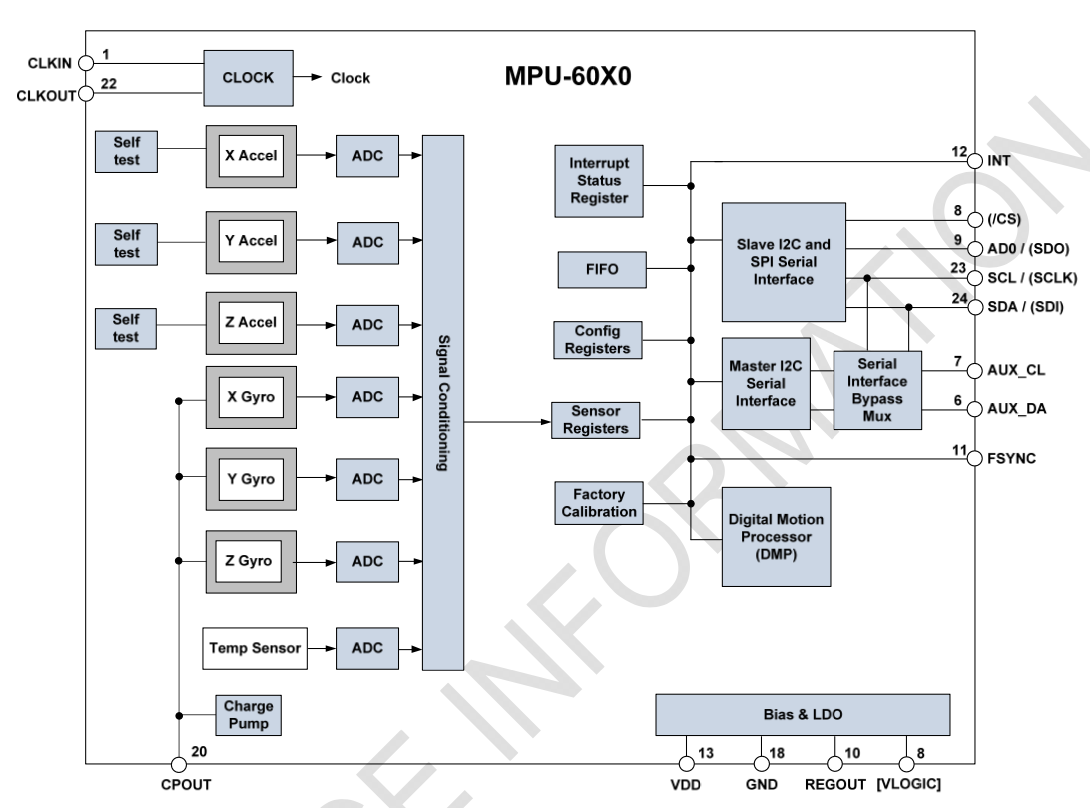
\includegraphics[width=0.8\textwidth]{img/mpu6050blockdiagram.png}
    \caption{GY 521 MOU 6050 Terminal Block Diagram\cite{mpu6050datasheet}}
    \label{fig:mpu6050blockdiagram}
\end{figure}

\begin{longtable}{|l|l|p{10cm}|}
\hline
\textbf{Pin Name} & \textbf{Pin Number} & \textbf{Description} \\ \hline
GND & 18 & Power supply ground. \\ \hline
VDD & 13 & Power supply voltage and digital I/O supply voltage. \\ \hline
CLKIN & 1 & Optional external reference clock input. Connect to GND if unused. \\ \hline
AUX\_DA & 6 & I2C master serial data, for connecting to external sensors. \\ \hline
AUX\_CL & 7 & I2C master serial clock, for connecting to external sensors. \\ \hline
VLOGIC & 8 (MPU-6050) & Digital I/O supply voltage. \\ \hline
AD0 / SDO & 9 & I2C Slave Address LSB (AD0); SPI serial data output (SDO). \\ \hline
REGOUT & 10 & Regulator filter capacitor connection. \\ \hline
FSYNC & 11 & Frame synchronization digital input. Connect to GND if unused. \\ \hline
INT & 12 & Interrupt digital output (totem pole or open-drain). \\ \hline
CPOUT & 20 & Charge pump capacitor connection. \\ \hline
CLKOUT & 22 & System clock output. \\ \hline
SCL / SCLK & 23 & I2C serial clock (SCL); SPI serial clock (SCLK). \\ \hline
SDA / SDI & 24 & I2C serial data (SDA); SPI serial data input (SDI). \\ \hline
NC & 2, 3, 4, 5, 14-17, 19, 21 & Not internally connected. May be used for PCB trace routing. \\ \hline
\caption{Terminal Function Table for MPU-6050\cite{mpu6050datasheet}}
\label{tab:terminal_functions}
\end{longtable}



\subsection{Magnetic Contactless Potentiometer - AS5600}

The AS5600 is an easy to program magnetic rotary position sensor with a high-resolution 12-bit analog or PWM output. This contactless system measures the absolute angle of a diametric magnetized on-axis magnet. This AS5600 is designed for contactless potentiometer applications and its robust design eliminates the influence of any homogenous external stray magnetic fields.\cite{AS5600Datasheet}


\textbf{Features:}
\begin{itemize}

    \item Contactless angle measurement
    \item Simple user-programmable start and stop positions over the I\textsuperscript{2}C interface
    \item Maximum angle programmable from 18 up to 360
    \item 12-bit DAC output resolution
    \item Analog output ratiometric to VDD or PWM-encoded digital output
    \item Automatic magnet detection
    \item Wide temperature range: -40 C to 125 C

\end{itemize}

\begin{figure}[ht]
    \centering
    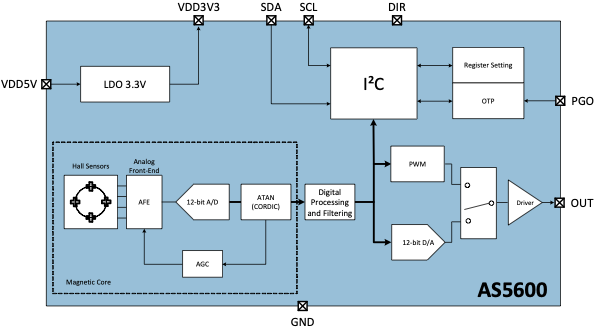
\includegraphics[width=0.6\textwidth]{img/magneticpotentiometerblockdiagram.png}
    \caption{Magnetic Contactless Potentiometer AS5600 Terminal Block Diagram\cite{AS5600Datasheet}}
    \label{fig:magneticpotentiometerblockdiagram}
\end{figure}

\begin{longtable}{|l|l|p{10cm}|}
\hline
\textbf{Pin Name} & \textbf{Pin Number} & \textbf{Description} \\ \hline
GND & 18 & Power supply ground. \\ \hline
VDD & 13 & Power supply voltage and digital I/O supply voltage. \\ \hline
CLKIN & 1 & Optional external reference clock input. Connect to GND if unused. \\ \hline
AUX\_DA & 6 & I2C master serial data, for connecting to external sensors. \\ \hline
AUX\_CL & 7 & I2C master serial clock, for connecting to external sensors. \\ \hline
VLOGIC & 8 (MPU-6050) & Digital I/O supply voltage. \\ \hline
AD0 / SDO & 9 & I2C Slave Address LSB (AD0); SPI serial data output (SDO). \\ \hline
REGOUT & 10 & Regulator filter capacitor connection. \\ \hline
FSYNC & 11 & Frame synchronization digital input. Connect to GND if unused. \\ \hline
INT & 12 & Interrupt digital output (totem pole or open-drain). \\ \hline
CPOUT & 20 & Charge pump capacitor connection. \\ \hline
CLKOUT & 22 & System clock output. \\ \hline
SCL / SCLK & 23 & I2C serial clock (SCL); SPI serial clock (SCLK). \\ \hline
SDA / SDI & 24 & I2C serial data (SDA); SPI serial data input (SDI). \\ \hline
NC & 2, 3, 4, 5, 14-17, 19, 21 & Not internally connected. May be used for PCB trace routing. \\ \hline
\caption{Terminal Function Table for MPU-6050\cite{mpu6050datasheet}}
\label{tab:terminal_functions}
\end{longtable}
\end{document}

\documentclass[english,project]{buwthesis}
\begin{document}
\chapter{Implementation}

This chapter describes the implementation process of the autonomous vehicle system, including hardware integration, software setup, and control algorithm. 

\section{Hardware Setup}

The hardware /setup involves the integration of several components to create the autonomous vehicle system. 
These components include the car (with pre-installed motor controller, circuit for remote control driving), Raspberry Pi 4,
Arduino Nano, LIDAR A1, 2 color sensors (TCS 34725), 1 motor driver (ZK BM1), 1 IMU sensor (MPU6050), a magnetometer (AS5600), and auxiliary components to build a robust hardware setup for testing. 
The auxiliary components include 2 breadboards, custom 3D-printed plates and LIDAR base, 11V LIPO battery, double-notch wires, external powered USB, rainbow wires, USB cables, simple strand wires, multimeter, LIPO and DC battery chargers, and LEGO components, glue gun, power bank. 
The listed items are exhaustive in order to provide clarity to reader for building a standalone system similar to the current configuration.


\subsection{Car Setup}
The vehicle is a compact car with the specifications descibred in the description of  Figure~\ref{fig:car}.


\sloppy
The car primary function is to be controlled through ROS2 nodes, enabling autonomous navigation, obstacle avoidance, 
and real-time sensor data response. The initial and final coordinates are published in order for car to locate 
its present location and for Nav2 stack localisation and path planning.
The vehicle has been modified to integrate sensors and computing units. 
More details on the custom car can be found in the manufacturer documentation \cite{BBH011_manual}
.

\subsubsection{Motor Control System}

\subsubsection{Steering Mechanism}
\sloppy
Unlike traditional toy autonomous vehicles that use stepper motors for steering, current vehicle in study uses a DC motor to control the front wheels. This introduces difficulty in precise angular positioning, leading to a hard steering effect. To mitigate this, the system initally had $-10.5^\circ$ to $+10.5^\circ$ range of motion with 5 steps, which later on converted to steering positions with 3 steps: extreme left, center, and extreme right.


\subsubsection{Power Distribution and Battery Management}

Power is supplied through:
\begin{itemize}
    \item A 12V 4.5 Ah DC battery for driving the motors
    \item An 11V LIPO battery for powering the computing and sensor units
    \item Optionally, a wall socket adapter can replace the LIPO battery for testing
    \item A power bank for exernal USB port in absence of wall socket.
\end{itemize}

The LIPO battery faces challenges in supplying sufficient power for remote operations. Consquently, for the last of project work, wall socket is preferred over LIPO.

\subsubsection{Sensor Placement and Data Fusion}

To achieve accurate navigation and obstacle avoidance, sensor placement is optimized:
\begin{itemize}
    \item LIDAR A1: Mounted at the rear for a stable 2D scan of the surroundings. The height is adjusted in order to prevent from any vision obstacle created by sensor installed on the car.
    \item IMU (MPU6050): Placed near the vehicle center to capture motion and orientation. The IMU sensor is oriented such that its $+x$ axis, marked on the device, is aligned parallel to the direction of the car's forward motion.

    \item Color Sensors (TCS 34725): One sensor positioned near a rear wheel for speed or distance estimation, the other near the front for steering feedback. The placement of color sensor on the steering wheel involves more work. Its included in the appendix \ref{chap:color_sensor}, for further information about the calculation and implementation. For now, we are not using color sensor for steering , problems are mention in he \ref{chap:color_sensor}. Morever, we are using the color sensor for measuring the steering wheel movement in which circle is dividing into 8 segments of black (each 40 degree) and 8 segments of white (each 5 degrees).The color sensor detects for the white color and each detection of white color measures to 8.125 cm for distance according to the circumference of the wheel of the car which is then used to calculate the odometery data.

    \begin{figure}[h!]
    \centering
    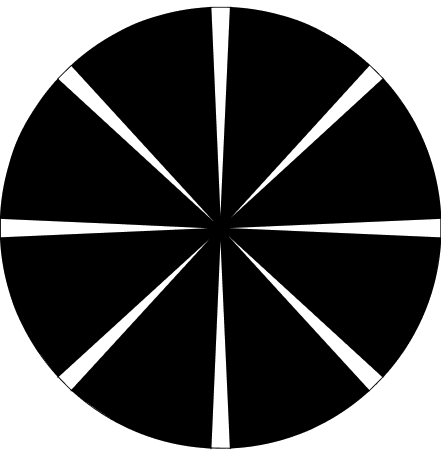
\includegraphics[width=0.6\textwidth]{img/implement/image.png}
    \caption{Design of wheel installed in the rear wheel}
    \label{fig:wiring_diagram}
    \end{figure}
    \item Magnetometer: It is used as an alternative for the measurement of why do we need to change from color to magentometer for measurement of steering wheel. Enhances orientation data, improving localization accuracy, placed on the steering wheel, however due to vertical movement of steering rod , distance b/w magnet and sensor is changing which causes noise in the steering data . This issue is still in To-Do list, more of it in discussion related to measurement of steering angle.
\end{itemize}

 \textbf{Problem 4:} The color sensor for steering feedback did not provide reliable data, requiring alternative placement or another sensor type.

\subsubsection{Chassis and Frame Design}

The car chassis balances weight distribution while accommodating all components efficiently. The frame is constructed from lightweight yet durable materials to maintain structural integrity. The compact size ensures maneuverability, which is crucial for indoor navigation and obstacle courses.


\subsubsection{Hardware to Software Communication using ROS2}

The data\textquotesingle s of system is structured into the following ROS 2 nodes:
\begin{itemize}
    \item /cmd\_vel: Publishes velocity commands.
    \item /scan: LIDAR publishes environmental scans.
    \item /imu: Publishes IMU data.
    \item /odom: Computes vehicle odometry. There is a custom node which combines the data of imu and color sensor to form odom.
\end{itemize}

This modular structure ensures flexibility and adaptability for future improvements.

\subsubsection{Future Enhancements and Reflection}

Planned improvements include:
\begin{itemize}
    \item Better Steering Control: Replacing the DC motor with a stepper motor.
    \item Power Optimization: Integrating more efficient battery management systems.
    \item Enhanced Navigation: Adding vision-based perception (e.g., cameras for SLAM and lane detection).
    \item Obstacle Avoidance Upgrades: Implementing ultrasonic sensors for close-range detection.


    %% changing rp4 to rp5.
    %% change steering to servo/stepper motor, which not involve any exernal sensor.
\end{itemize}

These enhancements will contribute to the long-term goal of making the vehicle more autonomous and robust in real-world applications.

\textbf{Note:} Open issues related to steering, battery limitations, and sensor feedback are discussed in section of Troubleshooting section.

%% if time and interest persists then i will write about the OPEN ISSUES.


\subsection{Raspberry Pi 4 Integration}
The Raspberry Pi 4 Model B serves as the main controller of the vehicle. It is equipped with the specifications discussed in the section of hardware details of Raspberry Pi 4.%% add cross-reference of rp4 section . 
 This system handles ROS2 communication, sensor integration, and motor control. The Raspberry Pi is responsible for reading data from the sensors (LIDAR, IMU, and color sensor) and sending control commands to the motor driver through arduino-nano.


\subsection{Diagrams for Wiring and Component Connections}
Detailed wiring diagrams are crucial for understanding how each component is interconnected within the system. These diagrams will include all connections related to power, data and control signals.

% Placeholder for the diagram
\begin{figure}[h!]
    \centering
    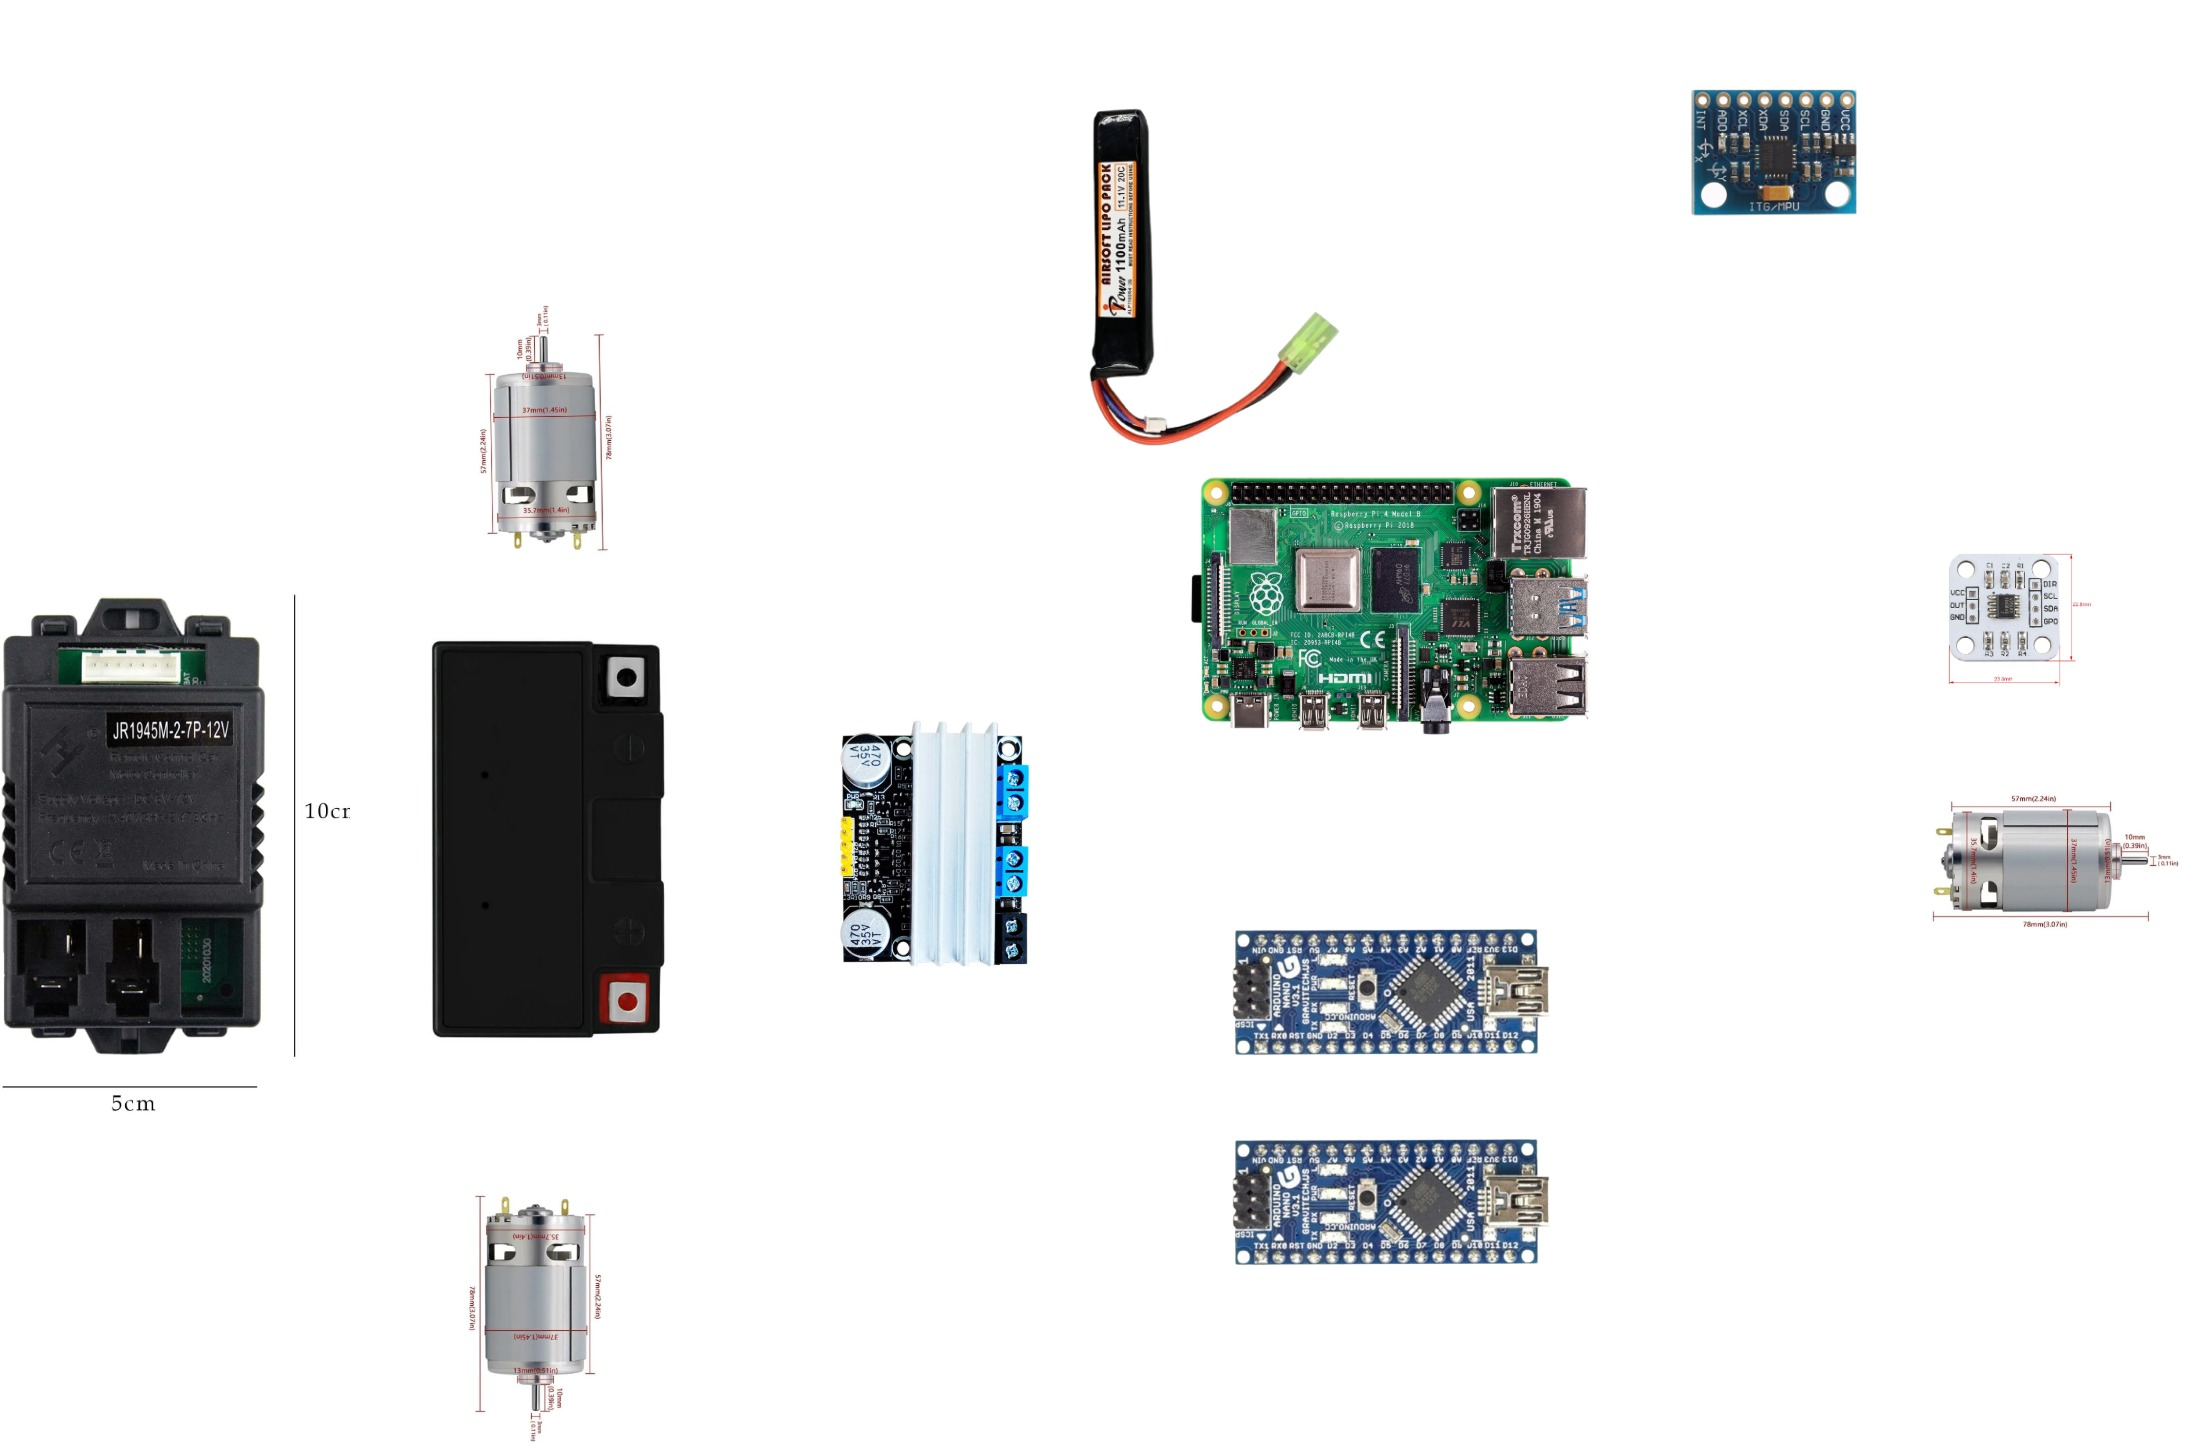
\includegraphics[width=\textwidth]{img/implement/Untitled Diagram-Page-1.jpg}
    \caption{Wiring Diagram of the Autonomous Vehicle System}
    \label{fig:wiring_diagram}
\end{figure}


\subsection{Photos of the Physical Setup}
Photos of the entire setup and close-ups of important components provide a visual understanding of the physical configuration of the autonomous vehicle.
% Placeholder for photos
\begin{figure}[h!]
    \centering
    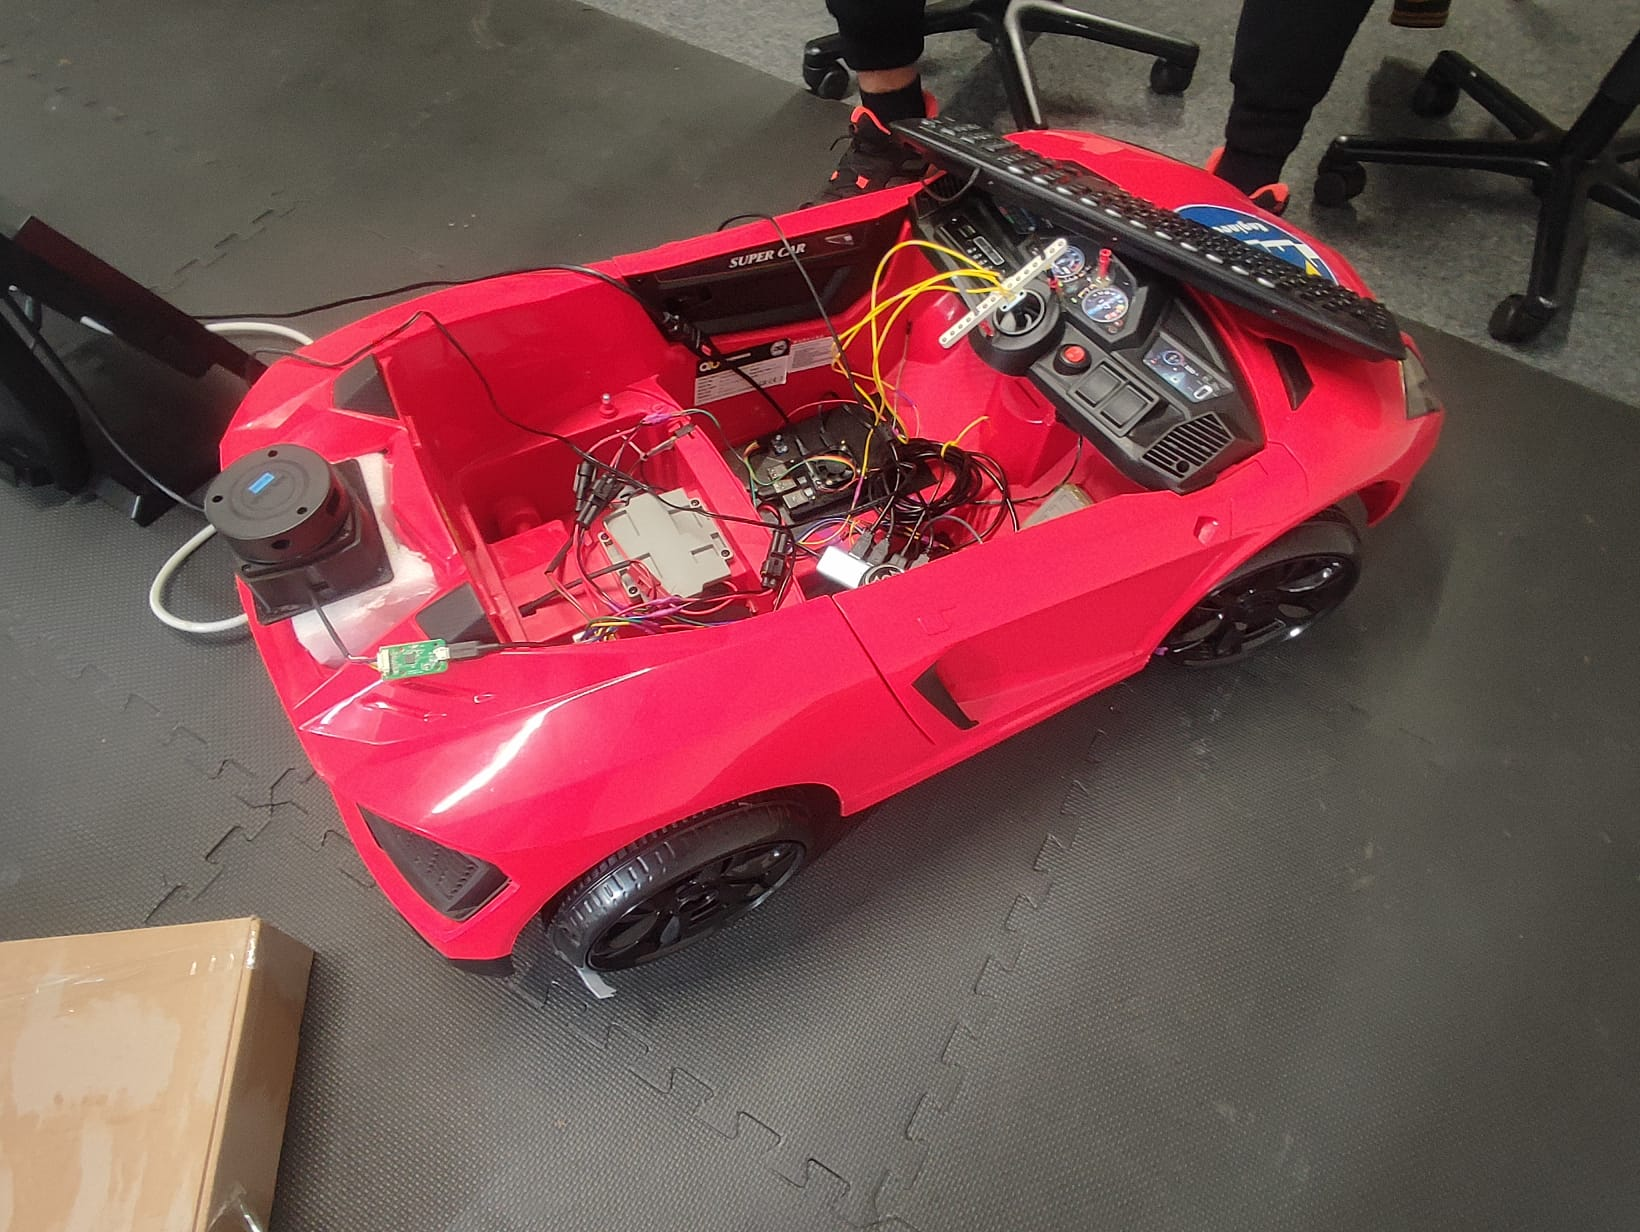
\includegraphics[width=\textwidth]{img/implement/WhatsApp Image 2025-03-08 at 7.44.38 PM.jpeg}
    \caption{Overall Setup of the Autonomous Vehicle}
    \label{fig:overall_setup}
\end{figure}

\subsection{Sensor and Motor Placement Diagrams}
Diagrams showing the placement of sensors and motors on the vehicle help in understanding their operational context and field of view.
% % Placeholder for sensor placement diagram
% \begin{figure}[h!]
%     \centering
%     \includegraphics[width=\textwidth]{path/to/sensor_placement_diagram.png}
%     \caption{Sensor and Motor Placement on the Vehicle}
%     \label{fig:sensor_placement}
% \end{figure}
% %% check ppt for this feature , take top view photo of car, use ppt feature to convert into skeleton form.


\subsection{Block Diagram for System Architecture}
A block diagram illustrating how various components such as sensors, processing units, and actuators are interconnected within the system.
% Placeholder for the block diagram
\begin{figure}[h!]
    \centering
    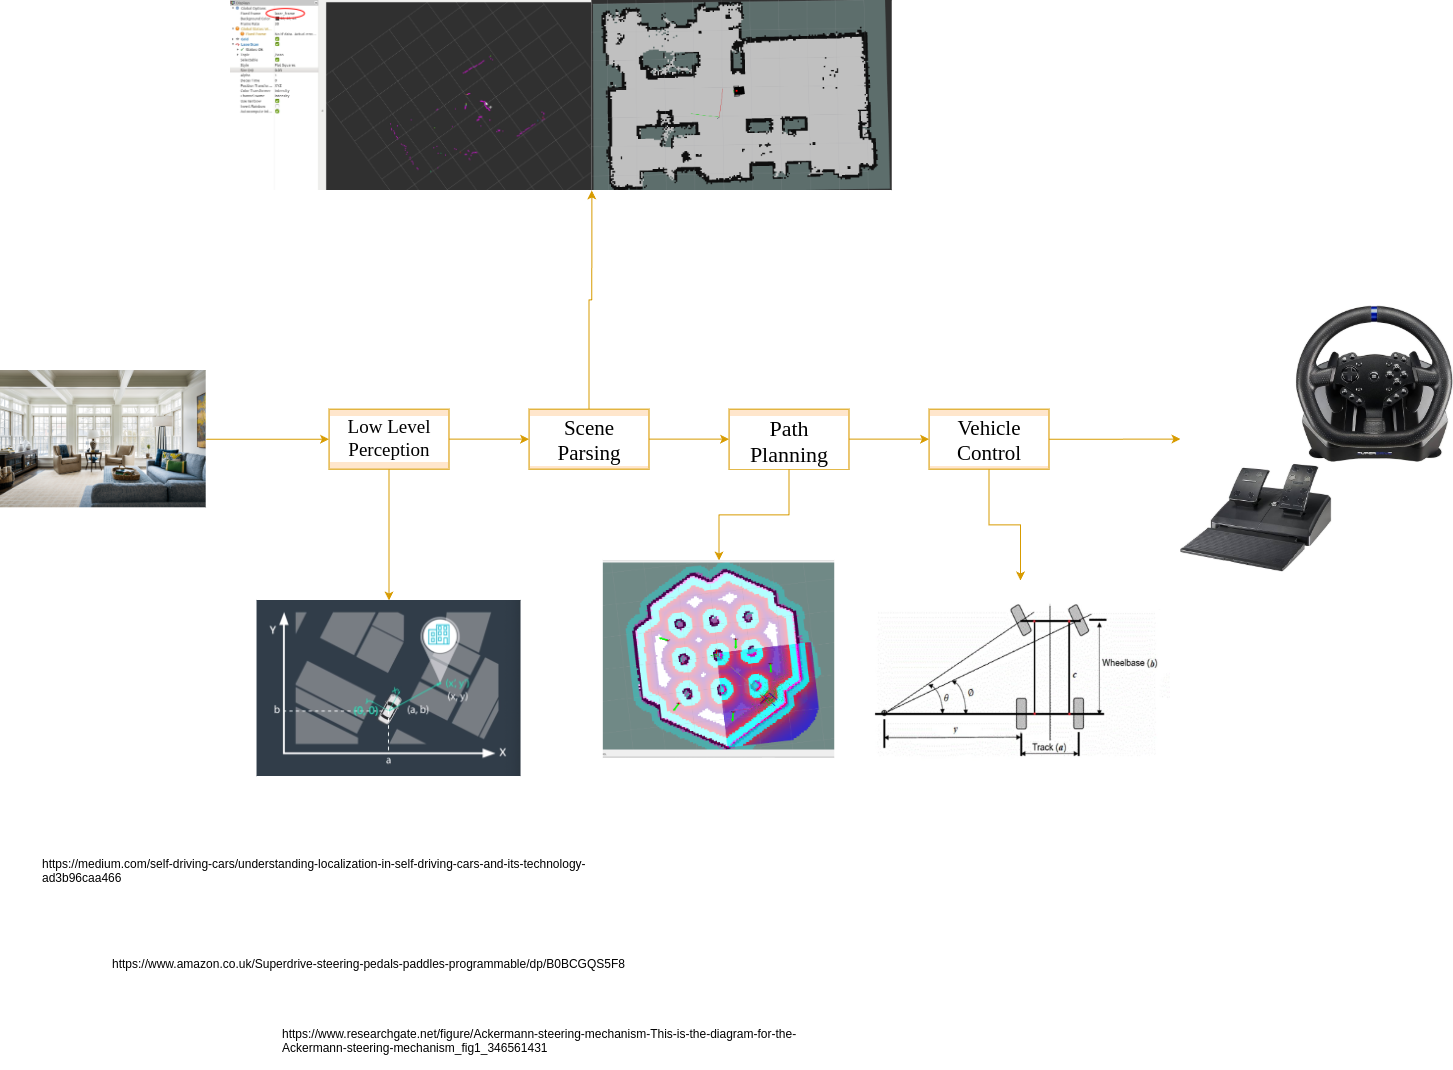
\includegraphics[width=\textwidth]{img/implement/high level architecture.png}
    \caption{System Architecture Block Diagram}
    \label{fig:system_architecture}
\end{figure}
% check draw.io page -3

\subsection{Power Consumption Analysis}
A detailed analysis of the power consumption of each component is essential to ensure the system operates efficiently without exceeding power supply capabilities. %% how to measure power consumption
% Placeholder for power consumption table
\begin{verbatim}
    | Component          | Power Consumption | Source     |
    |--------------------|-------------------|------------|
    | Raspberry Pi 4     | 5W                | LIPO       |
    | Arduino Nano       | 2W                | Power Bank |
    | LIDAR              | 1.5W            | Power Bank |
    | DC Motor Driver    | 15W               | DC battery |
    | Total              | 23.5W             |            |
\end{verbatim}


\subsection{Arduino Nano Integration}
\sloppy
An Arduino Nano is used to interface with the motor driver and manage motor control. The Arduino Nano is programmed to read PWM signals from the Raspberry Pi and control the speed and direction of the motors. The connection between the Raspberry Pi and the Arduino is done via a USB cable, and the Arduino is programmed to read the PWM signals and convert them into motor commands.


\subsection{Communication Protocols}

The hardware architecture relies on various communication protocols to ensure efficient data exchange between the Raspberry Pi, Arduino Nano, and the sensors. In this project, two primary interfaces are used: \textbf{I\textsuperscript{2}C} and \textbf{Serial UART}. The choice of protocol depends on factors such as available pins, data rate requirements, and ease of integration within the ROS2 framework.

\subsubsection{I\textsuperscript{2}C Communication}

I\textsuperscript{2}C (Inter-Integrated Circuit) is used for low-speed, short-distance, intra-board communication. It is a two-wire interface consisting of:
\begin{itemize}
    \item \textbf{SDA (Serial Data Line)}
    \item \textbf{SCL (Serial Clock Line)}
\end{itemize}

In this setup:
\begin{itemize}
    \item \textbf{IMU Sensor (GY-521 / MPU6050)}: Connected to the Raspberry Pi via I\textsuperscript{2}C for continuous accelerometer and gyroscope data.
    \item \textbf{Color Sensors (TCS34725)}: Operate over I\textsuperscript{2}C to send RGB and clear light intensity values. One sensor is used for measuring wheel speed (rear wheel), while the other attempts to provide steering feedback (although this remains problematic as noted in \textbf{Problem 4}).
    \item \textbf{Magnetometer (if applicable)}: Typically also integrated over I\textsuperscript{2}C to provide orientation data. Proper calibration and filtering are crucial for reliable measurements.
\end{itemize}

The Raspberry Pi 4\textquotesingle s I\textsuperscript{2}C pins (GPIO 2 for SDA and GPIO 3 for SCL by default) handle data traffic. Pull-up resistors are required on the I\textsuperscript{2}C lines (often provided on breakout boards). Each device on the bus has a unique address, and the Raspberry Pi acts as the master.

\subsubsection{Serial (UART) Communication}

Serial UART interfaces may be used for devices or debugging tools where a straightforward, point-to-point link is sufficient. Examples include:
\begin{itemize}
    \item \textbf{Arduino Nano Connection}: In some configurations, the Arduino Nano is connected to the Raspberry Pi via a USB-to-Serial interface. This allows the Raspberry Pi to send motor commands (e.g., PWM values) and receive any status messages from the Arduino.
    \item \textbf{Debugging Tools}: Occasionally, a USB-to-UART cable may be used for real-time debugging of sensor data or motor driver behavior.
\end{itemize}

While many sensors can use UART (e.g., some variants of GPS modules or other external boards), the core set of sensors in this project primarily rely on I\textsuperscript{2}C.

\subsubsection{Data Flow within ROS2}

Once the sensor data is received on the Raspberry Pi, it is published to the corresponding ROS2 topics. Key topic examples include:
\begin{itemize}
    \item \textbf{/imu} for accelerometer and gyroscope data from the MPU6050.
    \item \textbf{/steering\_sensor} or equivalent for color-sensor-based steering feedback.
    \item \textbf{/lidar\_scan} for the RPLIDAR A1 data (if using serial connection directly from LIDAR to the Pi).
\end{itemize}

Meanwhile, commands destined for the Arduino (such as motor speed control) flow from a ROS2 node on the Pi through the USB-to-Serial connection. This modular communication strategy keeps sensor processing and motor actuation neatly separated, and the ROS2 topics act as a flexible backbone for the exchange of information across the system.

% \subsubsection{Future Considerations}
% \begin{itemize}
%     \item \textbf{Network Communication}: Some modules (e.g., cameras or advanced LiDARs) might communicate over Ethernet or Wi-Fi, especially if more intensive data streams or remote monitoring are required.
%     \item \textbf{Protocol Optimization}: Tuning I\textsuperscript{2}C clock speed, ensuring minimal bus length, and reducing electrical noise can improve reliability. Proper cable management and shielding become more important as speed or distance increases.
% \end{itemize}

This layered approach, combining I\textsuperscript{2}C for sensor data acquisition and Serial for motor control and debugging, provides a balance between simplicity, scalability, and cost-effectiveness for an autonomous vehicle of this scale.
\begin{figure}[h!]
    \centering
    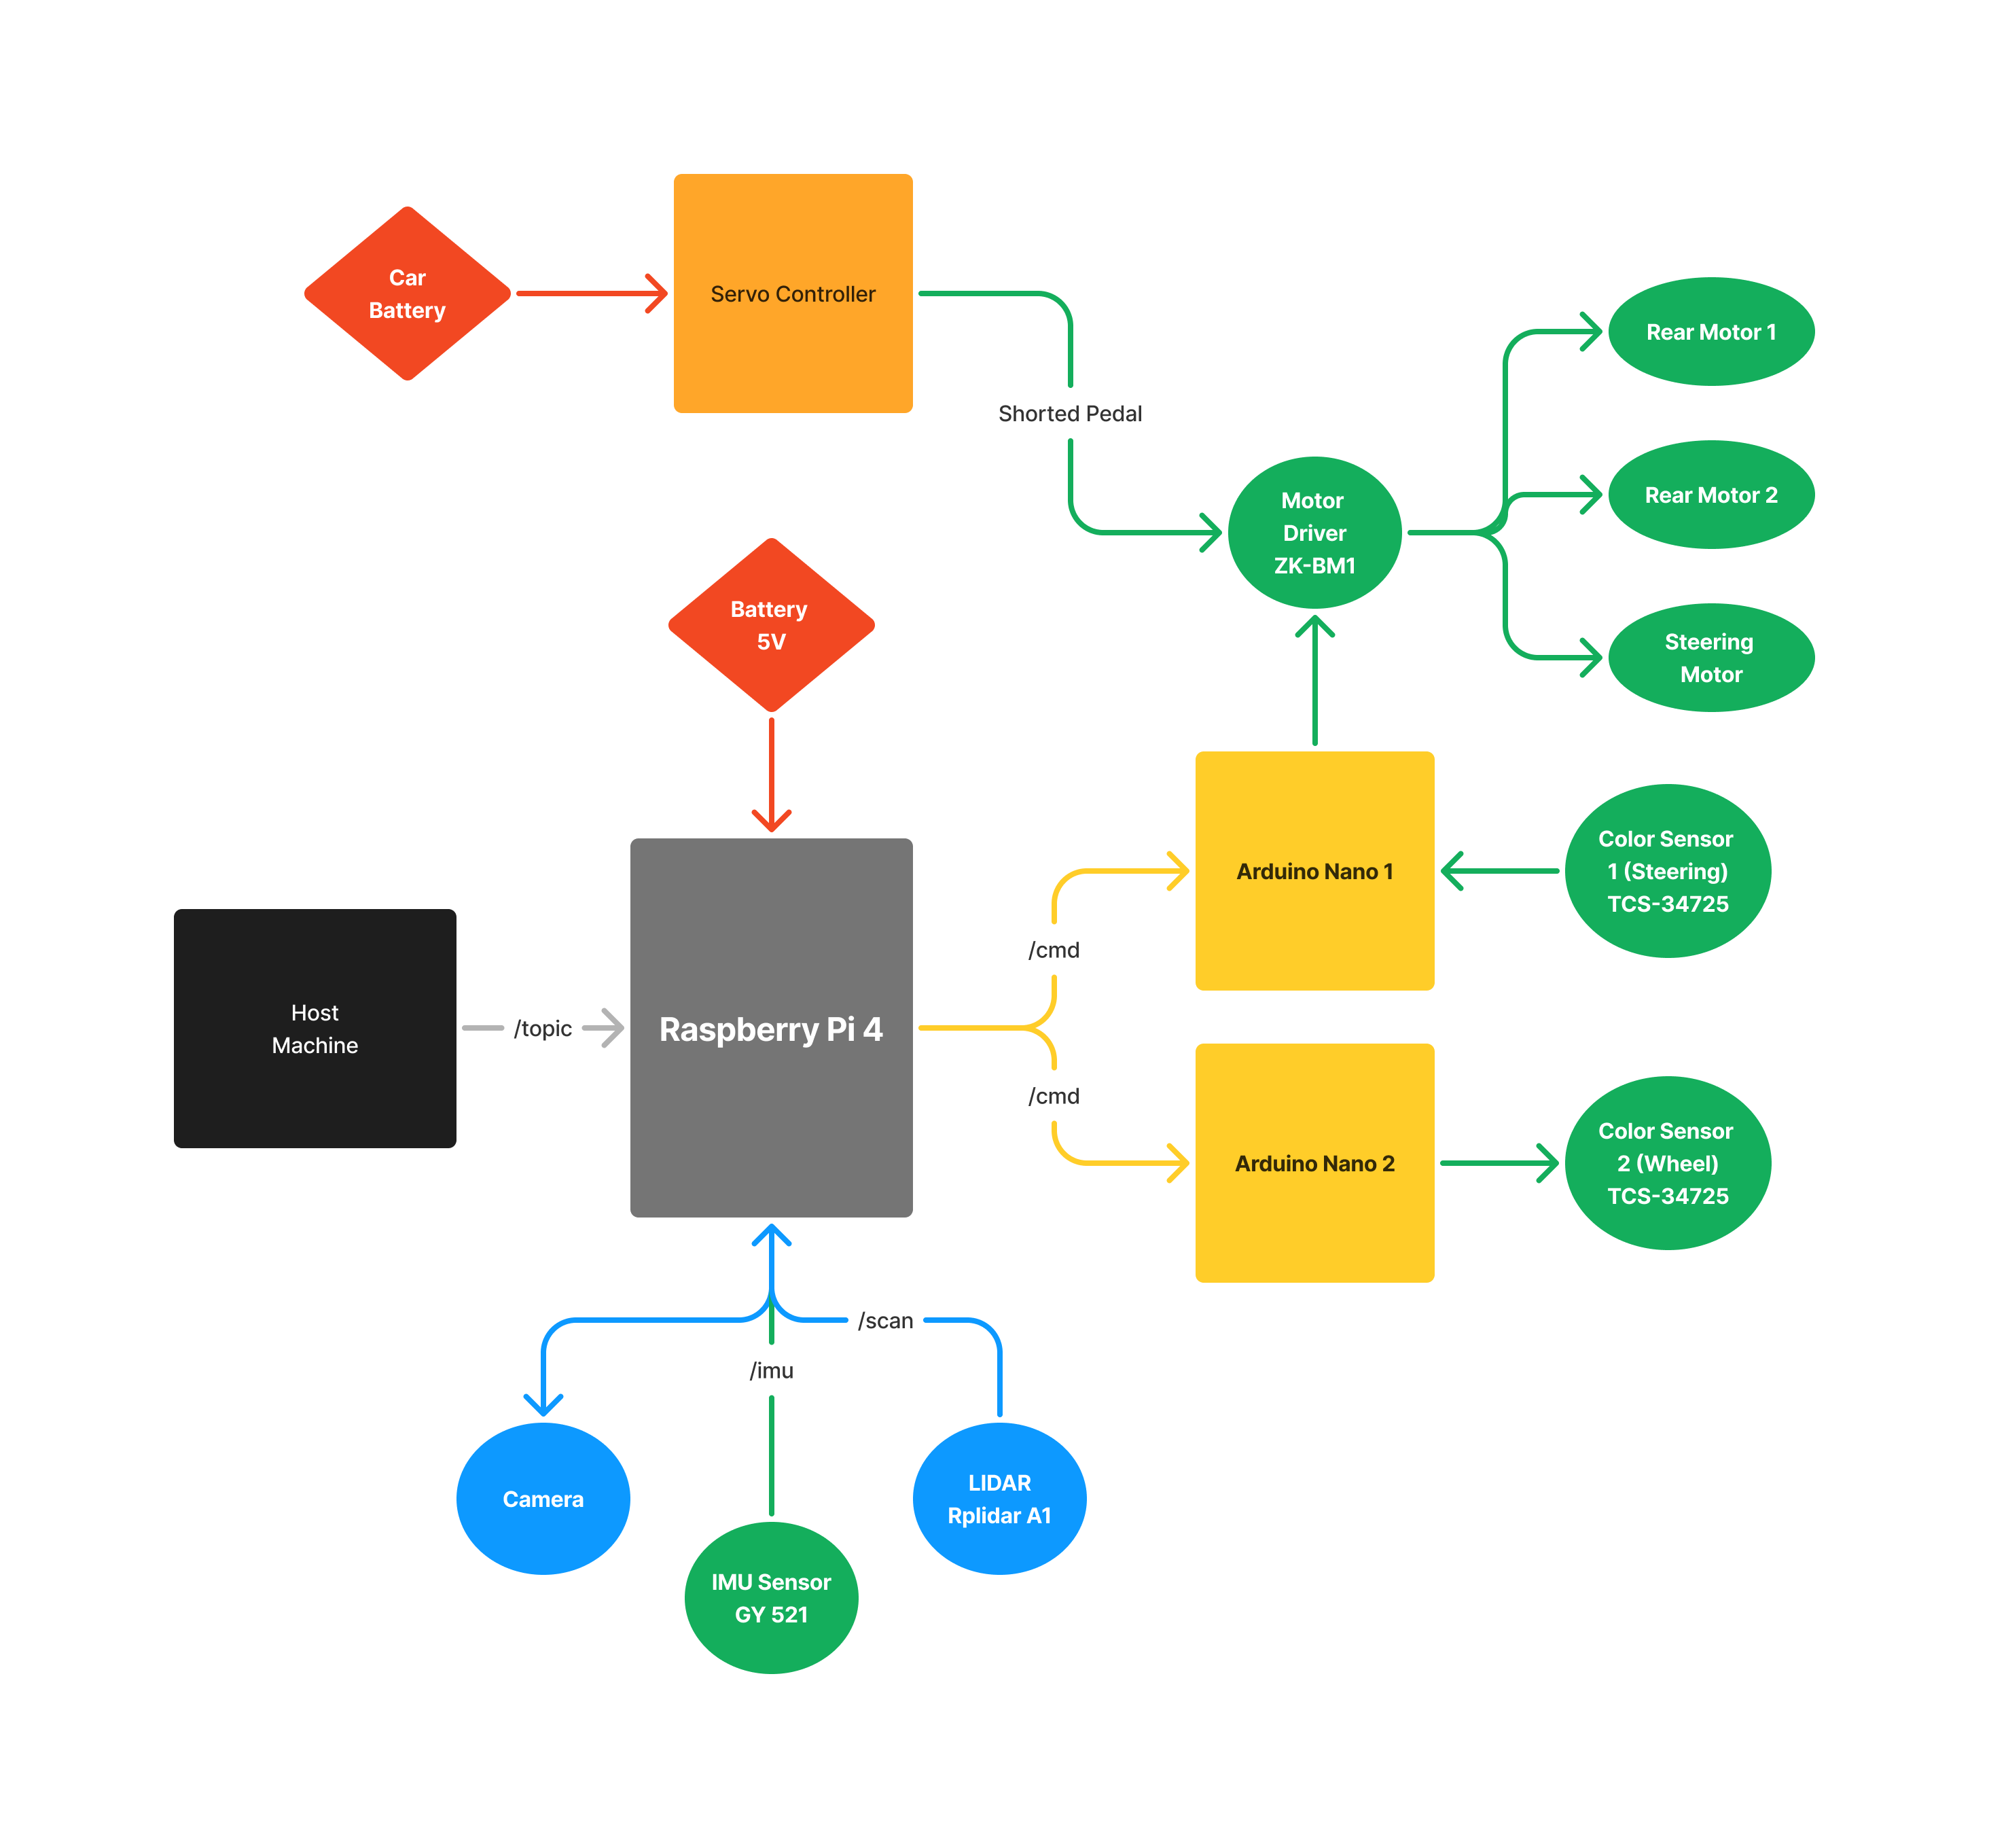
\includegraphics[width=\textwidth]{img/implement/Circuit Diagram(1).png}
    \caption{Overview diagram of hardware and communication}
    \label{fig:system_architecture}
\end{figure}
\subsection{Sensor Integration}
The system uses several sensors to provide data for navigation and control:
\begin{itemize}
    \item RPLIDAR A1: A 360-degree laser scanner used for environment mapping and localization.
    \item Color Sensor (TCS34725): This sensor provides RGB and clear light sensing, useful for detecting lines or specific objects for the vehicle's navigation.
    \item IMU Sensor (GY-521): The GY-521 sensor, based on the MPU6050, provides accelerometer and gyroscope data to estimate the vehicle's orientation and velocity.
\end{itemize}
These sensors are connected to the Raspberry Pi and communicate via I2C or serial communication protocols. 

\section{Software Setup}
The software stack is based on ROS2 Humble and is structured to ensure efficient communication between nodes and real-time control. The ROS2 setup involves several packages for sensor integration, control, and navigation.
%% add a digarm of nodes here and software architecture, topics in which msg is published, use something from rqt
\subsection{ROS2 Nodes}
The main nodes in the system include:
\begin{itemize}
    \item Sensor Nodes: These nodes handle data collection from the LIDAR, IMU, and color sensor. They publish the sensor data to relevant topics (e.g., `/scan`, `/imu/data`).
    \item Motor Control Node: This node receives velocity and steering commands and translates them into PWM signals for the motor driver via the Arduino.
    \item Navigation Nodes: These nodes are responsible for path planning and obstacle avoidance using the Nav2 stack.
\end{itemize}
\begin{figure}[h!]
    \centering
    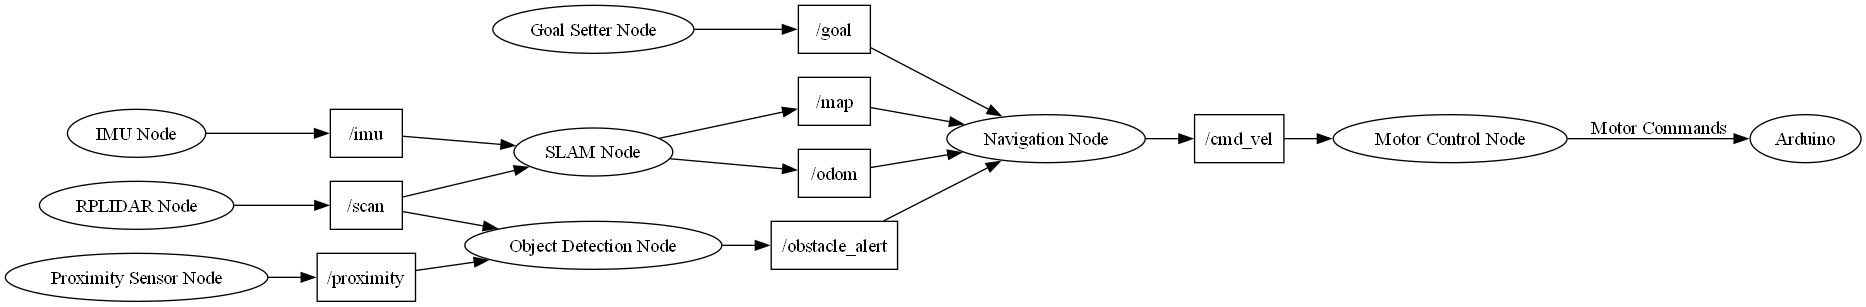
\includegraphics[width=\textwidth]{img/implement/ros2_communication_flow.png}
    \caption{Simplified Node Communication Schematic}
    \label{fig:system_architecture}
\end{figure}

\begin{figure}[h!]
    \centering
    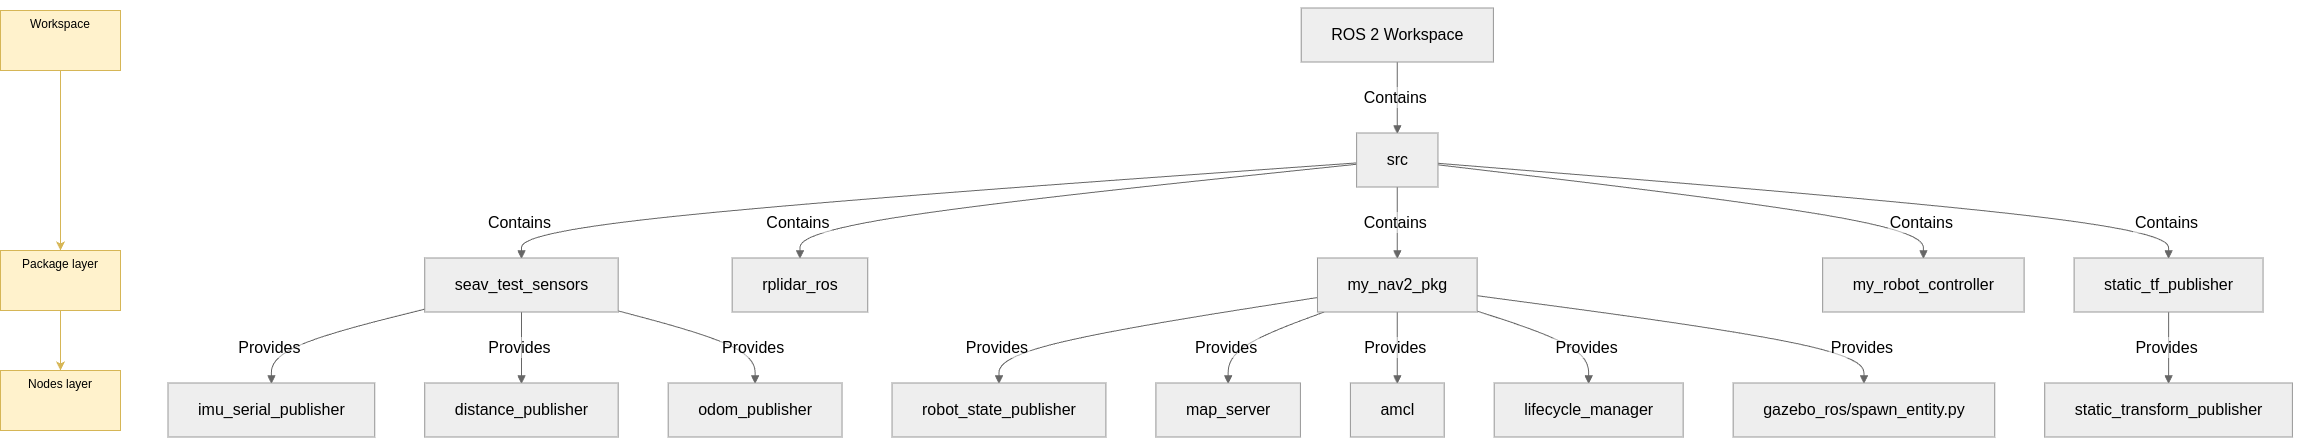
\includegraphics[width=\textwidth]{img/implement/layers and workspace.drawio.png}
    \caption{Workspace overview of pkgs built for the toycar}
    \label{fig:system_architecture}
\end{figure}
\subsection{Nav2 Setup}
Nav2 (Navigation 2) is configured to handle both global and local path planning. The main components of Nav2 include:
\begin{itemize}
    \item Global Planner: The global planner is responsible for planning the overall path from the start point to the goal. In this implementation, the A* algorithm is used for global path planning.
    \item Local Planner: The local planner adjusts the vehicle's trajectory in real-time, avoiding obstacles. The DWB (Dynamic Window Approach) planner is used for local path planning.
    \item Localization: The system uses the LIDAR and IMU data for localization, integrating these sensors with the AMCL (Adaptive Monte Carlo Localization) package to estimate the vehicle's position on the map.
    \item Costmaps: The global and local planners are informed by the costmaps, which represent the environment and obstacles. These costmaps are updated in real-time based on the LIDAR and IMU data.
\end{itemize}
\begin{figure}[h!]
    \centering
    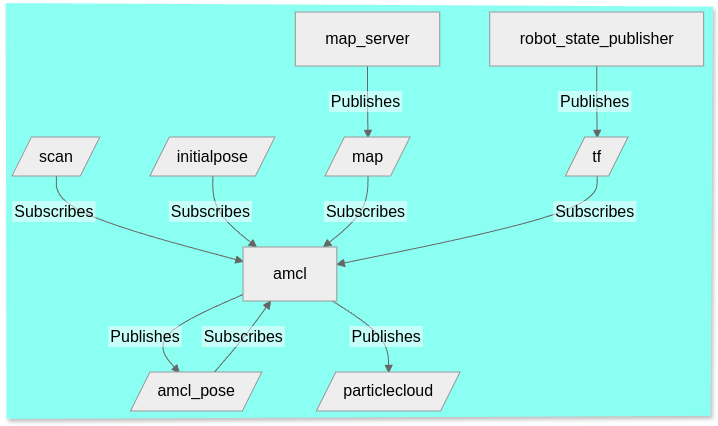
\includegraphics[width=\textwidth]{img/implement/amcl.drawio.png}
    \caption{AMCL Node}
    \label{fig:system_architecture}
\end{figure}


\begin{figure}[h!]
    \centering
    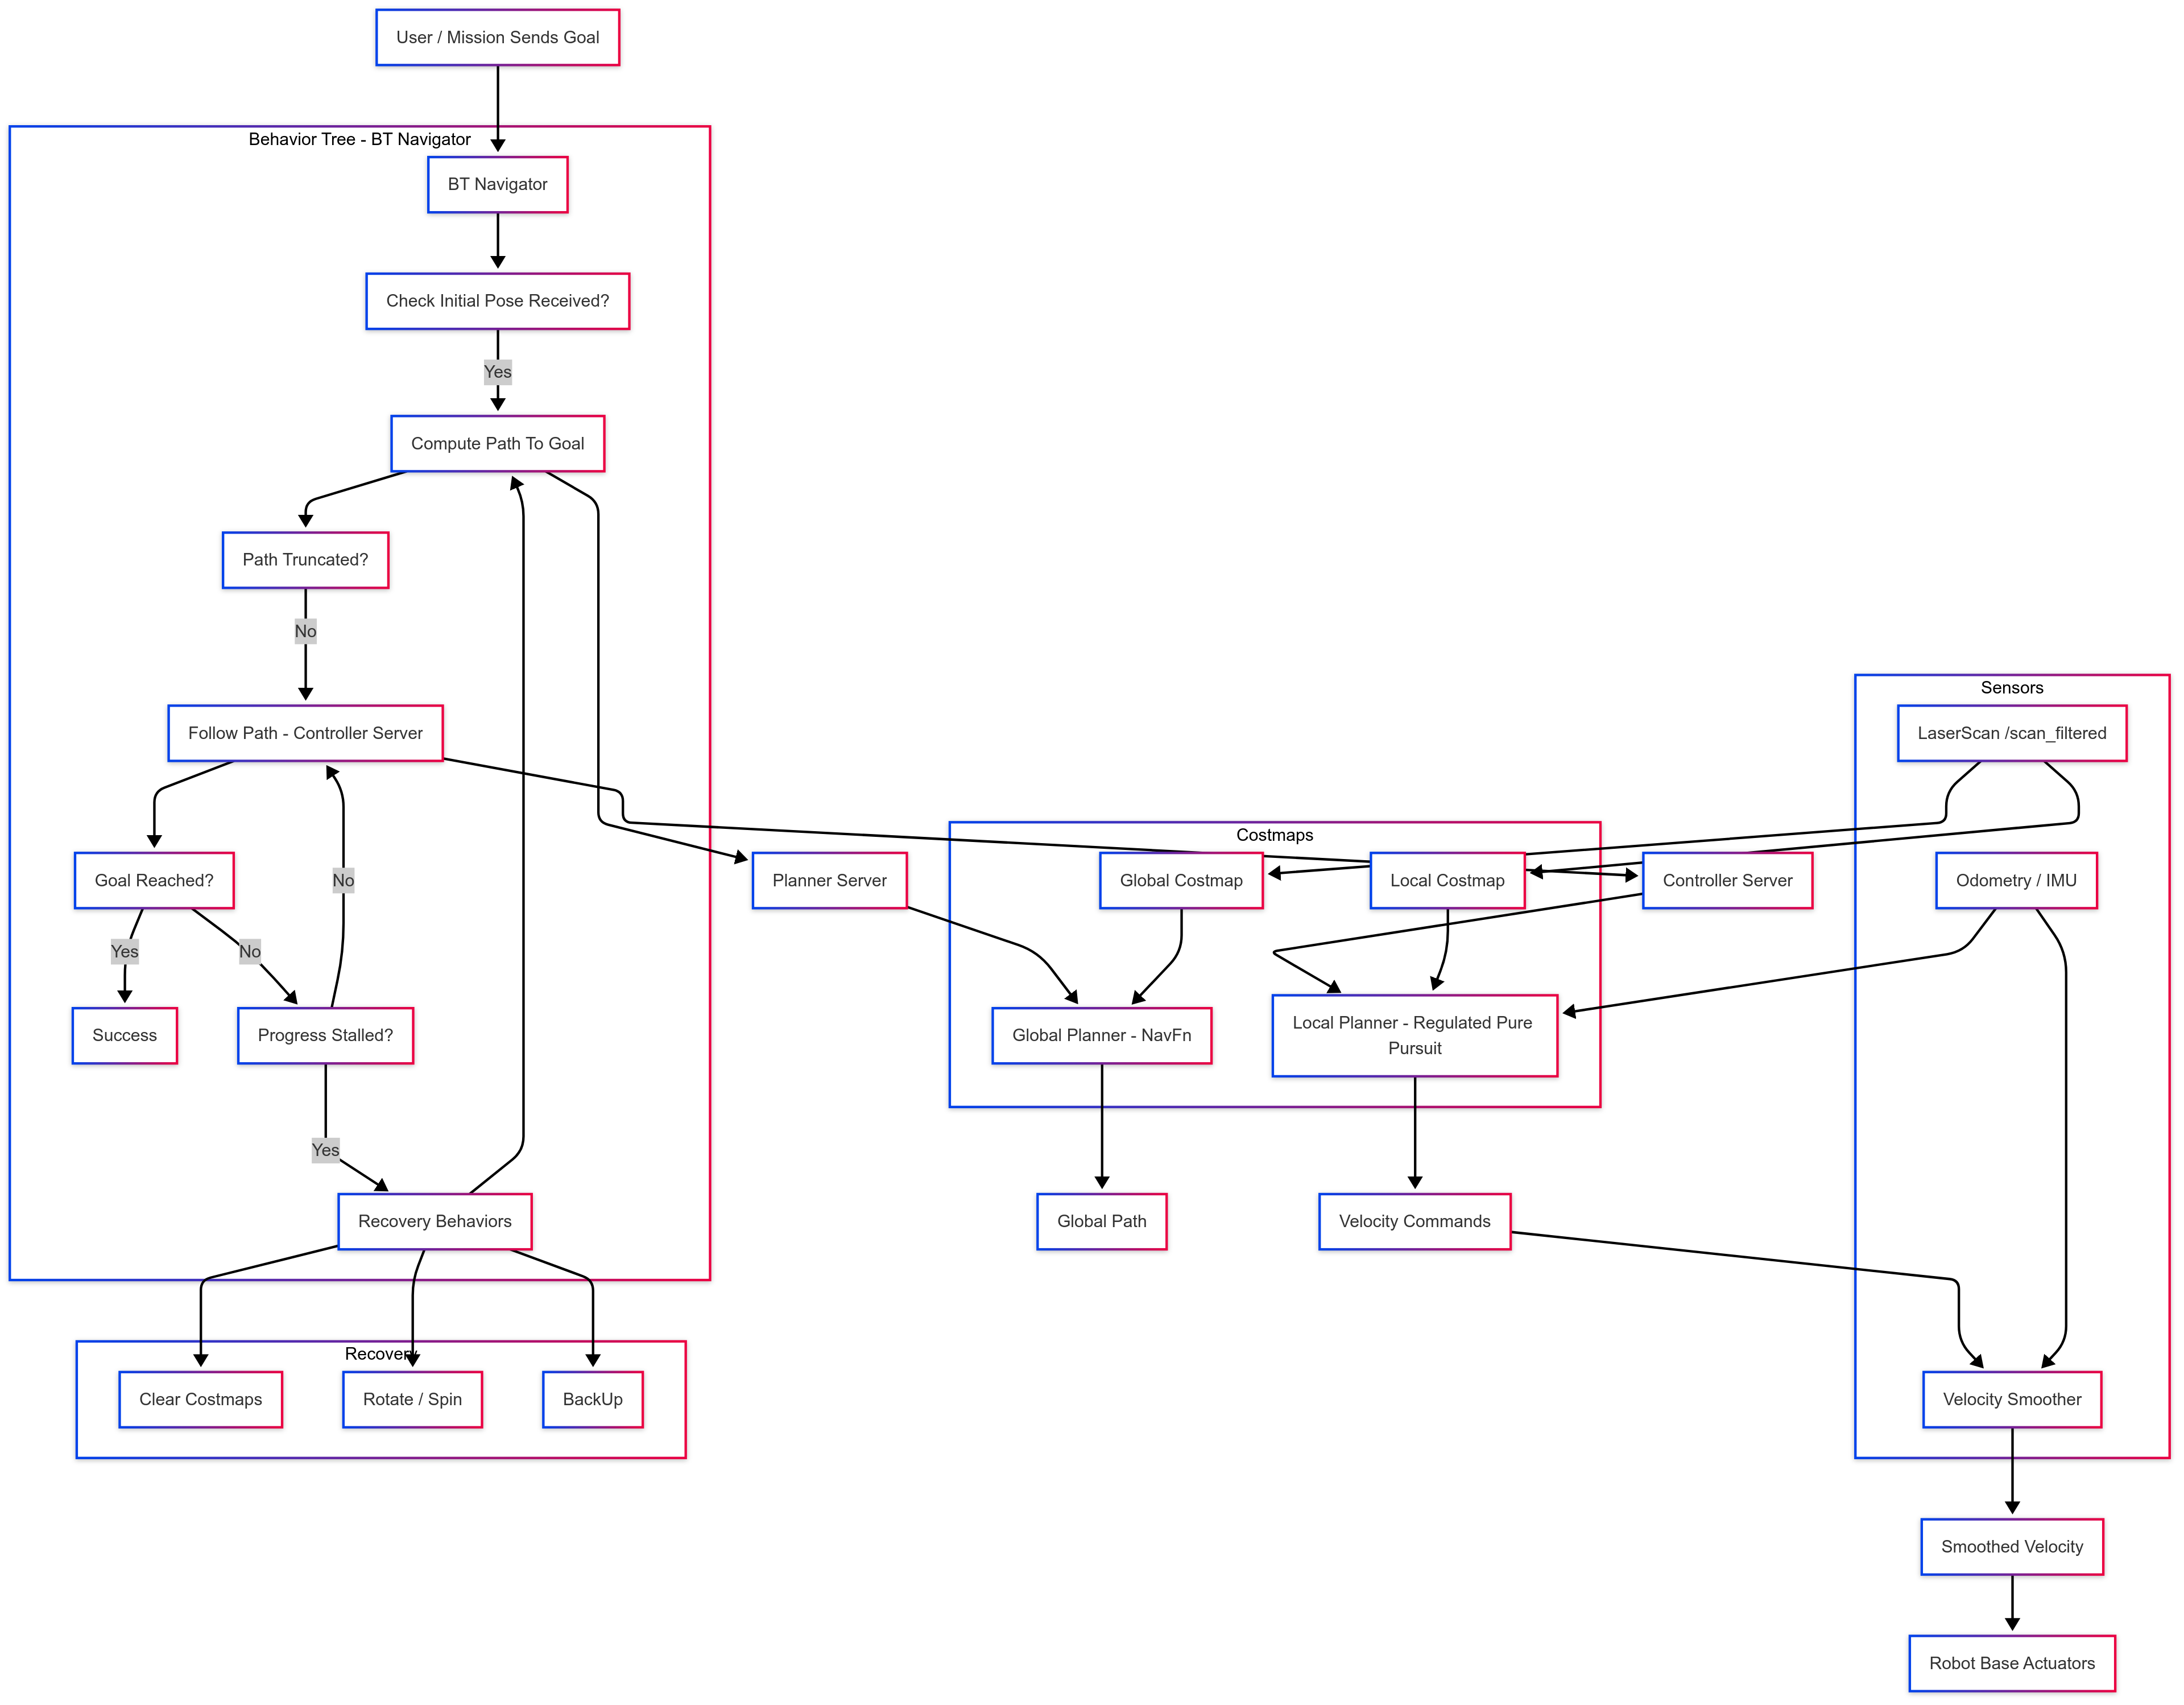
\includegraphics[width=\textwidth]{img/result/Nav2 autonomous decision making.png}
    \caption{Nav2 Autonomous Decision-Making Flow}
    \label{fig:system_architecture}
\end{figure}

\subsection{Controller}


\subsubsection{ros2 control}

\subsubsection{PID Controller}

\subsection{System Integration and Testing}
The system was integrated and tested in a controlled environment. The following steps were followed:
\begin{itemize}
    \item Hardware Integration: The Raspberry Pi, Arduino, motor driver, and sensors were connected and tested individually to ensure proper functionality.
    \item Software Integration: The ROS2 nodes were integrated to handle communication between components. Sensor data was published to topics, and motor control commands were sent to the motor driver.
    % \item **System Testing**: The system was tested in an indoor environment with a predefined path. The vehicle was able to follow the path and avoid obstacles based on the sensor feedback and the control algorithms.

    %% disucss for system testing topic for pre-defined path with Fazil
\end{itemize}
Testing was done with various scenarios to evaluate the system's robustness and performance in dynamic environments.

\subsection{Simulation and Testing in Gazebo}
Gazebo was used as the primary simulation environment to test and validate the software components before deploying them on the real autonomous vehicle. Simulation allows for controlled experiments, reducing the risk of hardware damage and enabling fine-tuning of algorithms.

\subsubsection{Vehicle Model in Gazebo}
To simulate the autonomous vehicle, a URDF (Unified Robot Description Format) and Xacro files were created. These files define the physical properties, kinematics, and dynamics of the car, including:
\begin{itemize}
    \item Wheelbase and track width dimensions to match the real vehicle.
    \item Definition of inertial properties for accurate physics simulation.
    \item Joint configurations for steering and rear-wheel drive motion.
    \item Sensor mount points for LIDAR, IMU, and color sensors.
\end{itemize}
The URDF model was loaded into Gazebo using the \texttt{robot\_state\_publisher} to ensure that the TF (Transform) tree was correctly defined for navigation.

\begin{figure}[ht]
    \centering
    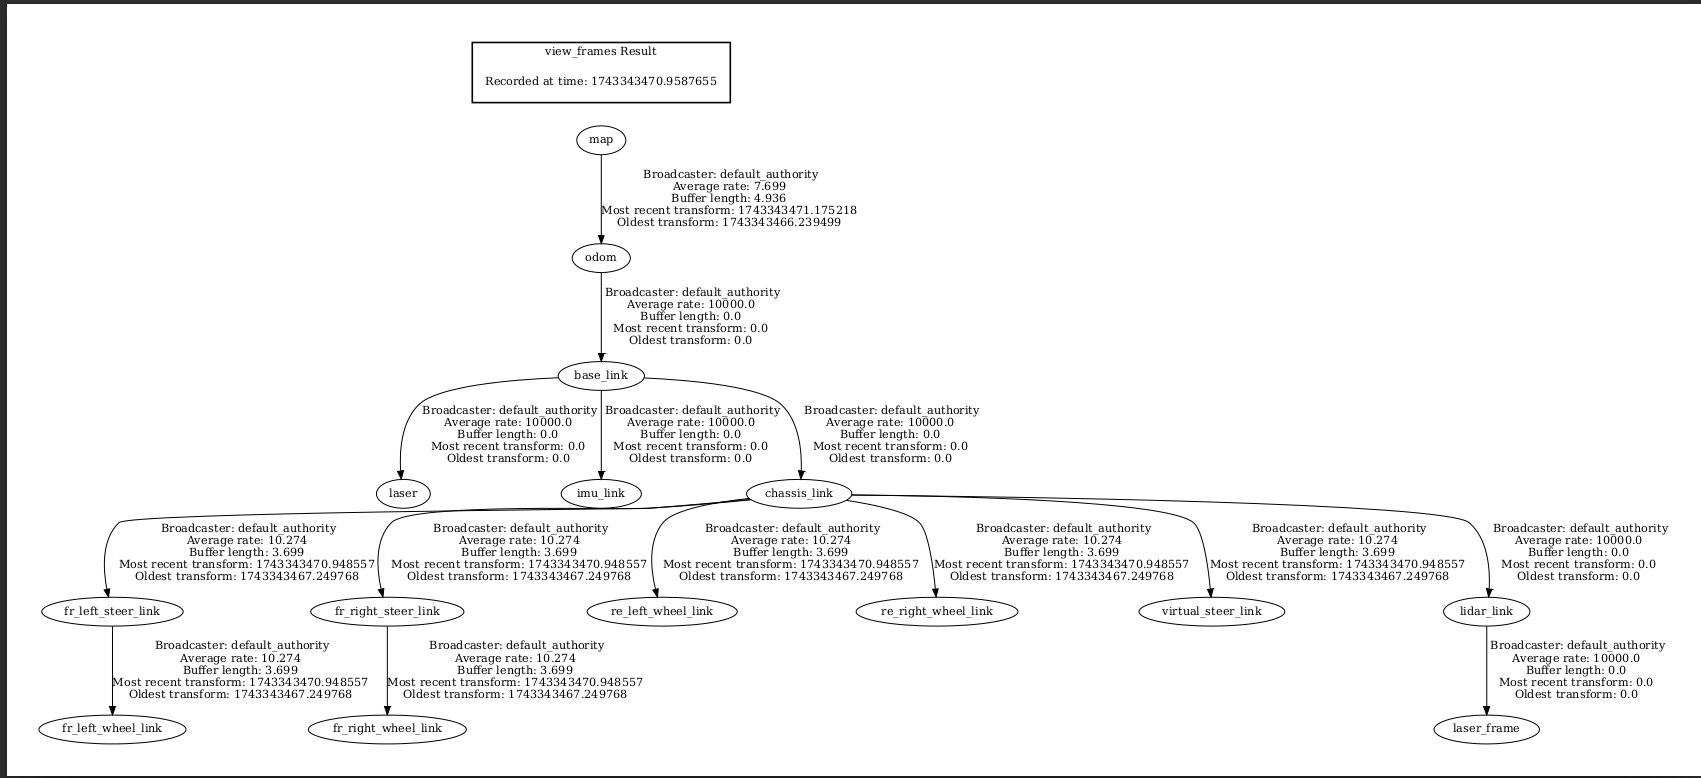
\includegraphics[width=0.8\textwidth]{img/result/tf_tree.jpg}  % No width scaling — uses original image size
    \caption{TF tree showing parent-child frame connections used by ROS transformations.}
    \label{fig:tf_tree}
\end{figure}


\subsubsection{Sensor Simulation}
Simulating the vehicle\textquotesingle s sensors within Gazebo was crucial for testing navigation algorithms. The following sensors were simulated:

\textbf{1. LIDAR Simulation:}
\begin{itemize}
    \item Implemented using the \texttt{gazebo\_ros\_ray\_sensor} plugin.
    \item Configured to publish scan data on the \texttt{/scan} topic.
    \item Used to test AMCL-based localization and SLAM mapping.
\end{itemize}


\textbf{2. IMU Simulation:}
\begin{itemize}
    \item The \texttt{gazebo\_ros\_imu\_sensor} plugin was used to generate \textbf{gyroscope and accelerometer data}.
    \item Data was published on the \texttt{/imu/data} topic to verify integration with \textbf{robot\_localization}.
\end{itemize}

%\textbf{2. IMU Simulation:}
%\begin{itemize}
%    \item The `gazebo_ros_imu_sensor` plugin was used to generate **gyroscope and accelerometer data**.
%    \item Data was published on `/imu/data` to verify integration with **robot_localization**.
%\end{itemize}

\textbf{3. Color Sensor Simulation:}
\begin{itemize}
    \item Since Gazebo lacks direct color sensor support, a custom Gazebo plugin was developed to mimic color detection based on object reflection properties.
    \item The color sensor was used to monitor the wheel rotation for odometry feedback.
\end{itemize}

\subsubsection{Currently testing Scenarios in Simulation}
Several scenarios were tested in Gazebo before real-world deployment:
\begin{enumerate}
    \item \textbf{Path Following:} The vehicle followed a predefined trajectory, validating motion control.
    \item \textbf{Obstacle Avoidance:} Objects were placed dynamically to evaluate the local planner's response to real-time obstacles.
    \item \textbf{SLAM Testing:} The vehicle explored an environment while generating a map using SLAM Toolbox.
    \item \textbf{PID Tuning:} Speed and steering PID controllers were adjusted iteratively in simulation to achieve smooth motion.
\end{enumerate}
Gazebo provided a realistic physics engine, enabling fine-tuned control over vehicle dynamics before real-world testing.

%% for gazebo based stuyd you can plenty of detail complete pipeline

\subsection{Debugging and Logging Strategies}
Effective debugging and logging are crucial for diagnosing issues and ensuring smooth operation of the ROS2-based autonomous vehicle. Several tools were employed to monitor node performance, sensor data accuracy, and real-time system behavior.

\subsubsection{ROS2 Logging}
ROS2 provides built-in logging mechanisms that allow developers to capture and analyze system behavior.

\textbf{Logging Strategies Used:}
\begin{itemize}
    \item Using \texttt{ros2 log}: Logs critical system events and errors during navigation.
    \item Logging severity levels: \texttt{Debug, Info, Warn, Error, and Fatal} were used to classify log messages.
    \item Redirecting logs to a file: 
    \texttt{\detokenize{ros2 launch <package_name> <launch_file>.launch.py --log-level debug > log.txt}}
\end{itemize}

\subsubsection{Data Visualization in RViz2 and Foxglove}
Visualization tools were essential for debugging sensor data and robot state.

%%%% https://docs.foxglove.dev/docs/connecting-to-data/frameworks/ros2, check foxglove good site

\textbf{1. RViz2 for ROS Visualization}
\begin{itemize}
    \item Used to visualize LIDAR scans, TF tree, costmaps, and AMCL localization.
    \item Allowed real-time inspection of `/tf` transformations and `/odom` data.
\end{itemize}

\textbf{2. Foxglove for Data Playback and Monitoring}
\begin{itemize}
    \item Enabled real-time analysis of ROS2 topics similar to \texttt{`rqt\_plot`}.
    \item Provided an interactive interface to inspect sensor readings.
\end{itemize}

\subsubsection{Performance Profiling and Optimization}
To ensure real-time operation, performance profiling tools were used:

\textbf{1. Topic Performance Analysis}
\begin{itemize}
    \item \texttt{ros2 topic hz /scan} -- Monitored LIDAR data publishing rate.
    \item \texttt{ros2 topic delay /cmd\_vel} -- Measured delays in command execution.
\end{itemize}

\textbf{2. Node Execution Time Profiling}
\begin{itemize}
    \item \texttt{ros2 run nav2\_util profiling\_tool} was used to measure computation times.
    \item Helped identify nodes with \textbf{high latency} and optimize computational efficiency.
\end{itemize}


\subsubsection{Error Handling and Recovery Mechanisms}
Various error-handling techniques were implemented to ensure robustness:
\begin{itemize}
    \item Node Failover: If a node crashes, automatic restart scripts were deployed using `systemd`.
    \item Watchdog Timer for Navigation: If no velocity command was published within a timeout period, the vehicle switched to a safe stop mode.
    \item Debugging IMU Drift: A low-pass filter was applied to IMU data to mitigate drift effects.
\end{itemize}

\subsection{Lessons Learned from Debugging}
Through extensive debugging and profiling, the following key improvements were made:
\begin{itemize}
    \item \textbf{Reduced Latency:} Optimized costmap updates to ensure smooth real-time navigation.
    \item \textbf{More Stable Localization:} Implemented sensor fusion between LIDAR and IMU for improved odometry.
    \item \textbf{Better Error Handling:} Introduced safety measures to prevent control system failures.
\end{itemize}

These enhancements significantly improved the \textbf{reliability and performance} of the autonomous vehicle system.

\subsection{Calibration Process}
To ensure accurate and reliable sensor measurements, the following calibration procedures were implemented:
\begin{itemize}
    \item LIDAR Calibration: Measured and adjusted for sensor alignment errors, ensuring precise distance measurements.
    \item IMU Calibration: Conducted bias correction and noise filtering to enhance orientation accuracy.
    \item Odometry Calibration: Measured wheel slip and encoder ticks to refine position estimation.
    \item Color Sensor Calibration: Tuned sensitivity to optimize color detection under different lighting conditions.
    \item Motor Controller Calibration: Adjusted PWM signals and motor response curves for smooth acceleration and deceleration.
\end{itemize}

\subsubsection{Troubleshooting and Challenges}
Throughout this project, several challenges arose that required systematic troubleshooting and problem-solving strategies. This section outlines the key difficulties encountered, the methods used to resolve them, and the lessons learned from these experiences. 

Each problem presented unique obstacles that required iterative testing, debugging, and optimization. By documenting these solutions, we not only improved the project\textquotesingle s robustness but also established a structured troubleshooting methodology for future enhancements.

\paragraph{Sensor Noise and Calibration Issues}
One of the earliest and most persistent challenges was dealing with sensor noise, particularly in the IMU and LIDAR data. Raw sensor readings exhibited fluctuations due to environmental factors, vibrations, and inherent measurement errors, leading to inconsistencies in localization and mapping.
\sloppy
To mitigate this:
\begin{itemize}
\item We implemented various filtering techniques such as:
  \begin{itemize}
    \item Low-pass filters to smooth out high-frequency noise in IMU acceleration and gyroscope data.
    \item Kalman filtering for optimal state estimation by fusing multiple sensor inputs, reducing drift, and improving real-time data reliability.
  \end{itemize}
\item Repeated calibration runs were performed using the Ferraris method to refine sensor parameters, ensuring more accurate and consistent readings. This involved:
  \begin{itemize}
    \item Performing controlled sensor movements and comparing results with ground truth data.
    \item Adjusting calibration parameters iteratively and re-evaluating error margins.
  \end{itemize}
\item Data logging and visualization tools were utilized extensively:
  \begin{itemize}
    \item Using ROS tools such as \texttt{rqt\_plot} and \texttt{rviz} to graphically analyze sensor data.
    \item Logging sensor outputs to CSV files and performing offline analysis to detect anomalies and optimize calibration parameters.
  \end{itemize}
\end{itemize}

\paragraph{Odometry Drift and Localization Errors}
Odometry drift was a significant challenge that impacted accurate navigation and map consistency over extended runs. In the present study, odometry (`/odom`) data is obtained by fusing measurements from two sensors: a color sensor mounted on the rear wheel and an Inertial Measurement Unit (IMU). The color sensor provides information regarding the linear distance traveled by the vehicle, calculated from the wheel rotation, while the IMU supplies angular velocity and linear acceleration data, facilitating accurate estimation of orientation, heading changes, and dynamic movements. By integrating these complementary data streams, odometry estimation is achieved, required for  localization and navigation performance. However the efficacy of the odom combination is not performed till now. the info about Wheel encoders, while useful, suffered from cumulative errors over time due to:
\begin{itemize}
\item Wheel slip, particularly on smooth surfaces, leading to incorrect distance measurements.
\item Uneven ground, affecting traction and introducing discrepancies in wheel odometry calculations.
\end{itemize}

To address this issue:
\begin{itemize}
\item We employed sensor fusion techniques, integrating data from multiple sources:
  \begin{itemize}
    \item Combining wheel odometry with IMU data to improve motion estimation.
    \item Implementing LIDAR-based SLAM (Simultaneous Localization and Mapping) to correct drift using environmental features.
  \end{itemize}
\item Regular calibration of wheel encoders was performed to reduce systematic drift errors:
  \begin{itemize}
    \item Conducting controlled movement tests over measured distances and adjusting encoder scaling factors accordingly.
    \item Logging odometry output and comparing with ground truth measurements to refine correction factors.
  \end{itemize}
\item Loop closure detection in SLAM was fine-tuned to correct accumulated drift over long-distance travel.
\item The TF (transform) tree structure in ROS was carefully verified to ensure consistent frame alignment between \texttt{odom}, \texttt{base\_link}, and sensor frames, preventing coordinate mismatches.
\end{itemize}

\paragraph{Motor Controller and PWM Signal Instability}
Motor control issues, such as erratic behavior and inconsistent speed regulation, were major obstacles in achieving smooth motion control. These issues were traced to:
\begin{itemize}
\item Noise and fluctuations in PWM signals affecting motor driver performance.
\item Insufficient resolution in duty cycle adjustments, leading to abrupt speed variations.
\item Power supply fluctuations impacting motor stability.
\end{itemize}

To resolve these problems:
\begin{itemize}
\item We fine-tuned PWM frequency and duty cycle values to achieve stable motor responses.
\item Debugging logs were introduced to monitor real-time motor control outputs, helping to diagnose inconsistencies.
\item We tested different motor driver configurations, adjusting voltage levels to prevent underpowering or overdriving.
\item A PID (Proportional-Integral-Derivative) controller was implemented for fine-grained speed regulation, ensuring smooth acceleration and deceleration.
\end{itemize}

\paragraph{Environmental Factors Affecting Sensor Performance}
LIDAR and color sensor performance was impacted by varying environmental conditions, including:
\begin{itemize}
\item Changes in ambient lighting affecting color sensor accuracy.
\item Surface reflectivity variations leading to LIDAR range errors.
\item External interference from nearby objects affecting sensor consistency.
\end{itemize}

Mitigation strategies included:
\begin{itemize}
\item Adjusting sensor placement and orientation to reduce interference and improve coverage.
\item Implementing adaptive thresholding for color sensors to dynamically adjust readings based on lighting conditions.
\item Conducting extensive testing across different environments to validate sensor robustness.
\item Using additional shielding and optical filters to reduce interference from ambient light and reflections.
\end{itemize}

\paragraph{Communication and Synchronization Issues}
Inter-node communication in ROS occasionally led to delays, affecting real-time performance. This was due to:
\begin{itemize}
\item High message frequency overloading the ROS network.

\item Inconsistent timestamps across different sensor topics leading to synchronization issues. We fixed the inconsistent timestamps across sensor topics by ensuring all messages included proper ROS time headers and aligning their publishing rates. We adjusted the `transform\_timeout` and `tf\_buffer\_duration` parameters in the SLAM configuration to handle minor timing differences. Additionally, we verified synchronization using the \textbf{SLAM precheck script}, ensuring all sensor timestamps were within an acceptable range before launching SLAM.
\end{itemize}


To resolve these:
\begin{itemize}
\item We optimized ROS topic frequencies to balance data rates and computational load.
\item Implemented time synchronization methods to align timestamps across different sensor nodes.
\item Debugging tools like \texttt{rostopic echo}, \texttt{rosbag} recording, and playback were used to analyze message delays and identify bottlenecks.
\end{itemize}

\paragraph{Peripheral and System-Level Challenges}
While these issues did not directly impact the project's core objectives, they significantly influenced development efficiency and workflow.

One such issue was configuring the Raspberry Pi 4 (RP4) for SSH connectivity. Initially, the built-in WiFi failed to establish a stable connection, preventing remote access. After multiple debugging attempts, we discovered that the default network manager settings conflicted with the SSH service. To resolve this:
\begin{itemize}
\item We manually configured the \texttt{/etc/wpa\_supplicant.conf} file with the correct WiFi credentials.
\item Restarted network services and tested connectivity using Ethernet to ensure SSH accessibility.
\item Updated system firmware to patch potential WiFi driver issues.
\end{itemize}

Another major setback was the choice of the operating system. We initially deployed the Ubuntu GUI version, but performance issues arose due to excessive resource usage, leading to system lag. To optimize performance:
\begin{itemize}
\item We switched to the Ubuntu CLI version, significantly reducing memory and CPU consumption.
\item Removed unnecessary background services and optimized boot configurations for headless operation.
\end{itemize}

Additionally, debugging hardware-related issues such as faulty SD cards, inconsistent power delivery, and peripheral failures required extensive testing. A key realization was that suboptimal power adapters led to undervoltage warnings, causing unexpected reboots. The final solution involved using a high-quality, 5V 3A power adapter to ensure system stability. Battery performance limitations also posed a challenge, as unexpected battery drain under load affected overall system uptime. We implemented voltage and current monitoring mechanisms to ensure stable power distribution and prevent sudden failures.
\sloppy
Furthermore, the Raspberry Pi 4 often experienced overheating issues
during extended operation, especially under heavy computational loads. 
We resolved this by installing a heat sink and an active cooling fan, which significantly improved thermal performance and prevented unexpected
thermal throttling. The integration of the ROS2 Control framework, 
specifically with the \texttt{ackermann\_steering\_controller}, introduced
additional complexity. Debugging motor command alignment with ROS2 Control 
commands required extensive tuning, particularly in ensuring real-time compliance with the ROS2 control loop rates. The lack of steering feedback
in early tests compounded these issues, leading to overshooting and
inaccurate angles. To address this, we explored the use of a color sensor
as a feedback mechanism, improving the accuracy of the steering response.
\sloppy
Another unexpected issue arose with the USB peripherals, where certain devices failed to initialize upon boot. This was traced back to power distribution inconsistencies across the USB ports. To mitigate this, we used externally powered USB hubs to provide stable voltage levels to connected devices, ensuring reliable performance. We also encountered difficulties with file system corruption, particularly when abrupt power losses occurred. To address this, we enabled journaling on the file system, implemented automated backups, and ensured the system used a UPS (Uninterruptible Power Supply) to prevent data loss in case of unexpected shutdowns.

In addition, the SLAM and mapping process presented significant challenges, particularly with .pgm map files. Issues arose in creating, loading, and interpreting maps, requiring careful tuning of parameters such as map resolution, inflation radius, and obstacle definitions to ensure accurate navigation. By systematically addressing these challenges, we significantly improved the reliability and accuracy of our system. The solutions developed in this project not only enhanced our understanding of robotic systems but also provided a structured approach for troubleshooting future projects.



\end{document}
\documentclass[english,project]{buwthesis}
\begin{document}
\chapter{Results}

In this section, we present the results obtained from the various tests and experiments conducted on the system. The system performance was evaluated across several key areas, including basic motion control, sensor integration, localization and path planning.

\subsection{Basic Motion and Steering Control}

The basic motion and steering control was tested using velocity commands sent through the command line interface. We validated the responsiveness of the motors and steering mechanism, ensuring that the vehicle could move forward, reverse, and turn accurately. The system initially operated in manual control mode, through keyboard and joystick and the transition to autonomous control is still ongoing.

%%should i describe about the node communication for running this car.
%% add simulatantoeus photo of fwd, left and right photo
% \begin{figure}[ht]
%     \centering
%     \includegraphics[width=0.7\textwidth]{motion_control.png}  % Replace with actual image
%     \caption{Test Setup for Basic Motion and Steering Control}
%     \label{fig:motion_control}
% \end{figure}

%% what kind of image can i add here ?

\subsection{Sensor Integration and Localization}
Sensor data integration is a critical component for achieving accurate localization and mapping in mobile robotics. In the present setup, localization is achieved by fusing data from an Inertial Measurement Unit (IMU) and a color-based distance sensor. These sensors work in tandem to estimate the robot\textquotesingle s position and orientation, enabling continuous publishing of the odometry (odom) information through a custom ROS 2 node.

The IMU provides angular velocity (yaw rate) data, which is integrated over time to estimate the robot\textquotesingle s heading or orientation ($\theta$). Simultaneously, the color sensor measures the distance traveled, which serves as an alternative to traditional wheel encoders. This distance information is used to estimate the robot\textquotesingle s position incrementally along the current heading.

The sensor fusion in this setup is implemented through deterministic dead reckoning. The angular velocity from the IMU is used to compute the change in heading, and this heading is combined with the latest distance reading to calculate updates to the robot\textquotesingle s $x$ and $y$ positions. This fusion process is executed at a fixed frequency (10 Hz), and the resulting pose and velocity estimates are published using the $nav_msgs/Odometry message$ type on the $/odom$ topic. At the same time, a tf2 transform between the odom and $base_link$ frames is broadcast to maintain frame consistency.

While this approach does not yet incorporate probabilistic filters such as an Extended Kalman Filter (EKF), it provides a lightweight and responsive method for estimating odometry in simple environments. The fusion node is also designed with time-critical constraints in mind, using a rolling TF2 buffer (0.1 seconds) to limit transform history and ensure fresh data publication. The implementation takes care to flush outdated TF data and uses reliable QoS settings to guarantee that odometry and transform messages are delivered accurately.




% \begin{figure}[ht]
%     \centering
%     \includegraphics[width=0.7\textwidth]{sensor_integration.png}  % Replace with actual image
%     \caption{LIDAR, IMU, and Color Sensor Data Integration}
%     \label{fig:sensor_integration}
% \end{figure}

\subsection{SLAM and Mapping}

SLAM was successfully implemented using IMU and LIDAR in a simulated environment. The vehicle was able to map its environment and localize itself within the map. However, the integration of dynamic obstacles for real-time mapping is still pending, and this is expected to improve the overall navigation system's performance in more complex environments.
    

\begin{figure}[H]
    \centering
    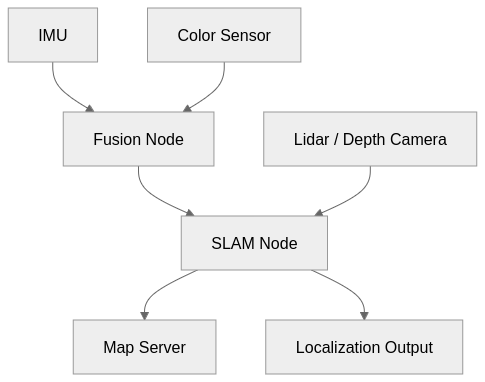
\includegraphics[width=0.7\textwidth]{img/result/slam.drawio.png}  % Replace with actual image
    \caption{Sensor fusion and SLAM pipeline. IMU and color sensor data are fused to generate odometry, which, together with Lidar data, is used by the SLAM node to compute both a map and the robot's estimated position.}
    \label{fig:slam_pipeline}
\end{figure}

\begin{figure}[ht]
    \centering
    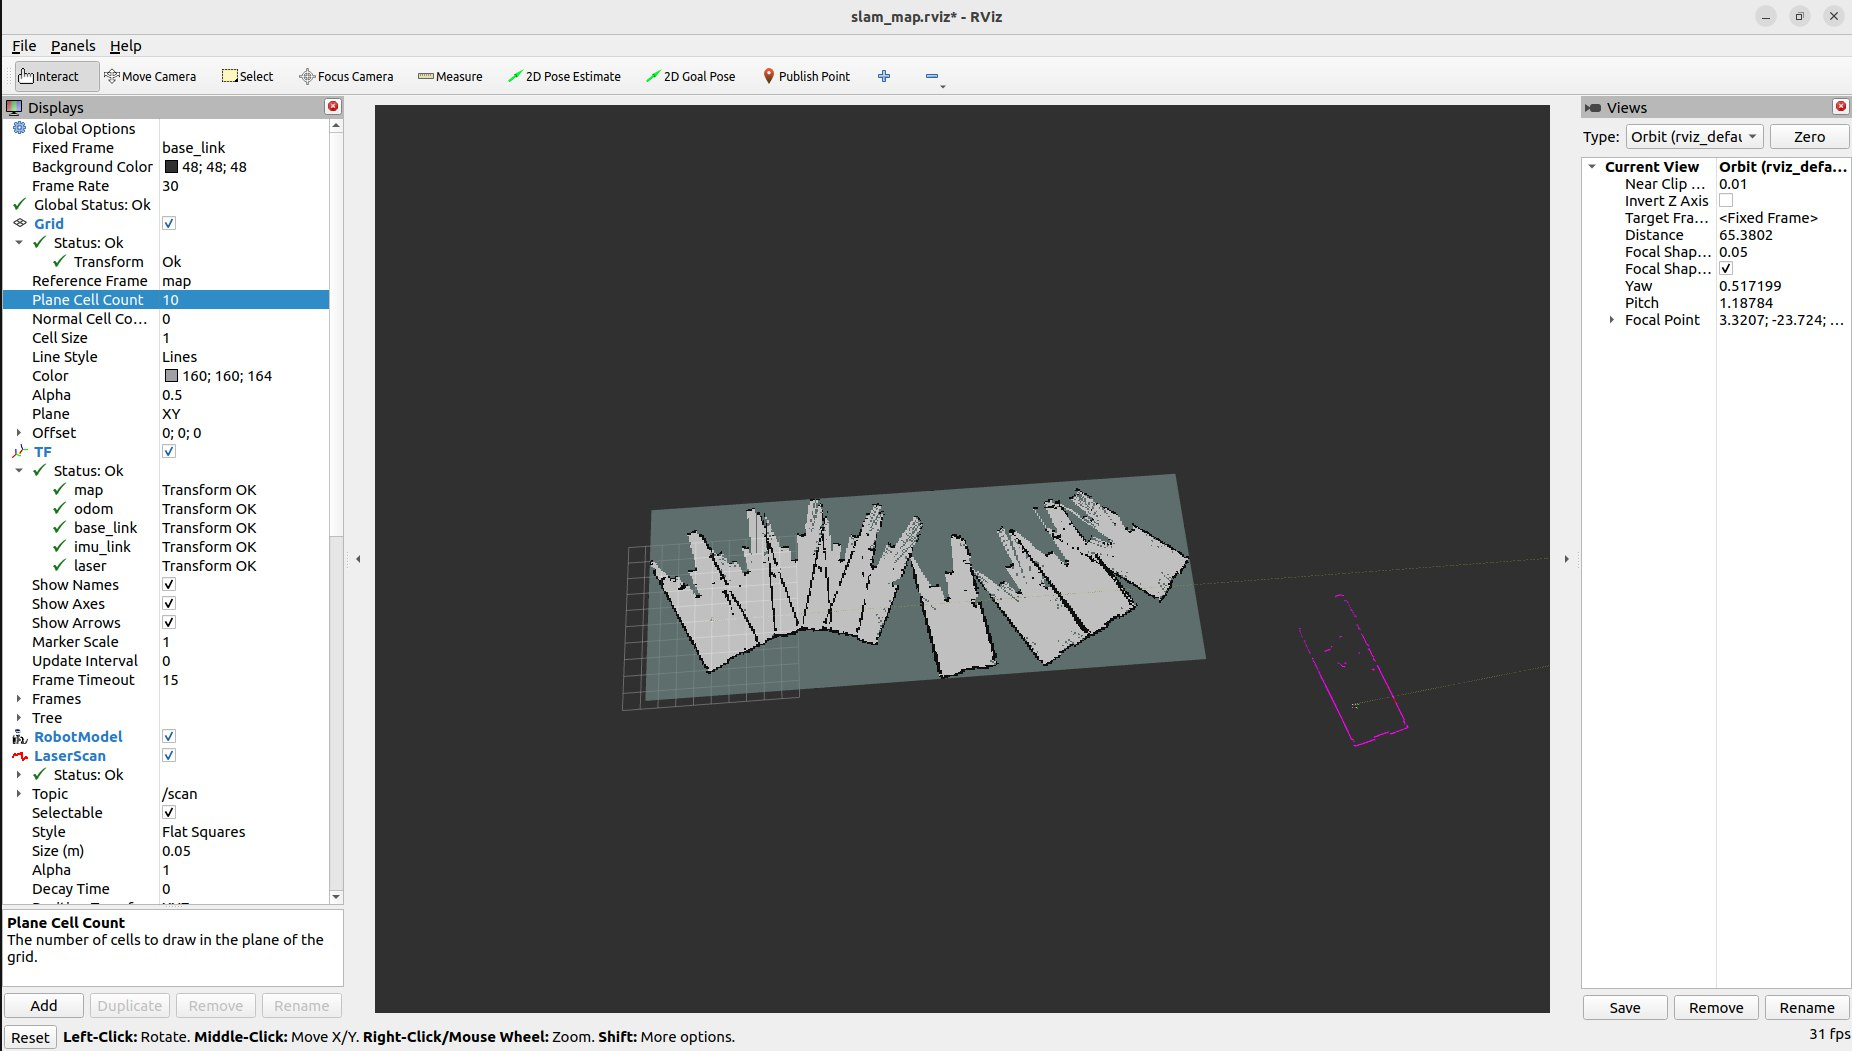
\includegraphics[width=0.7\textwidth]{img/result/slam_before_imu.jpeg}  % Replace with actual image
    \caption{SLAM map}
    \label{fig:slam map generated before imu calibration}
\end{figure}

\subsection{Path Planning and Navigation}

The goal-setting and navigation functionality using Nav2 was successfully tested with mock maps. The system could generate feasible paths for the robot to navigate from a starting point to a destination. Further testing with real sensor data and dynamic environments is required to refine the system\textquotesingle s performance.

In terms of dynamic path planning and obstacle avoidance, the Gazebo simulation allowed us to test the basic functionality. However, the real-time updates and the ability to adapt to sudden changes in the environment are still areas for improvement.

\begin{figure}[h]
    \centering
    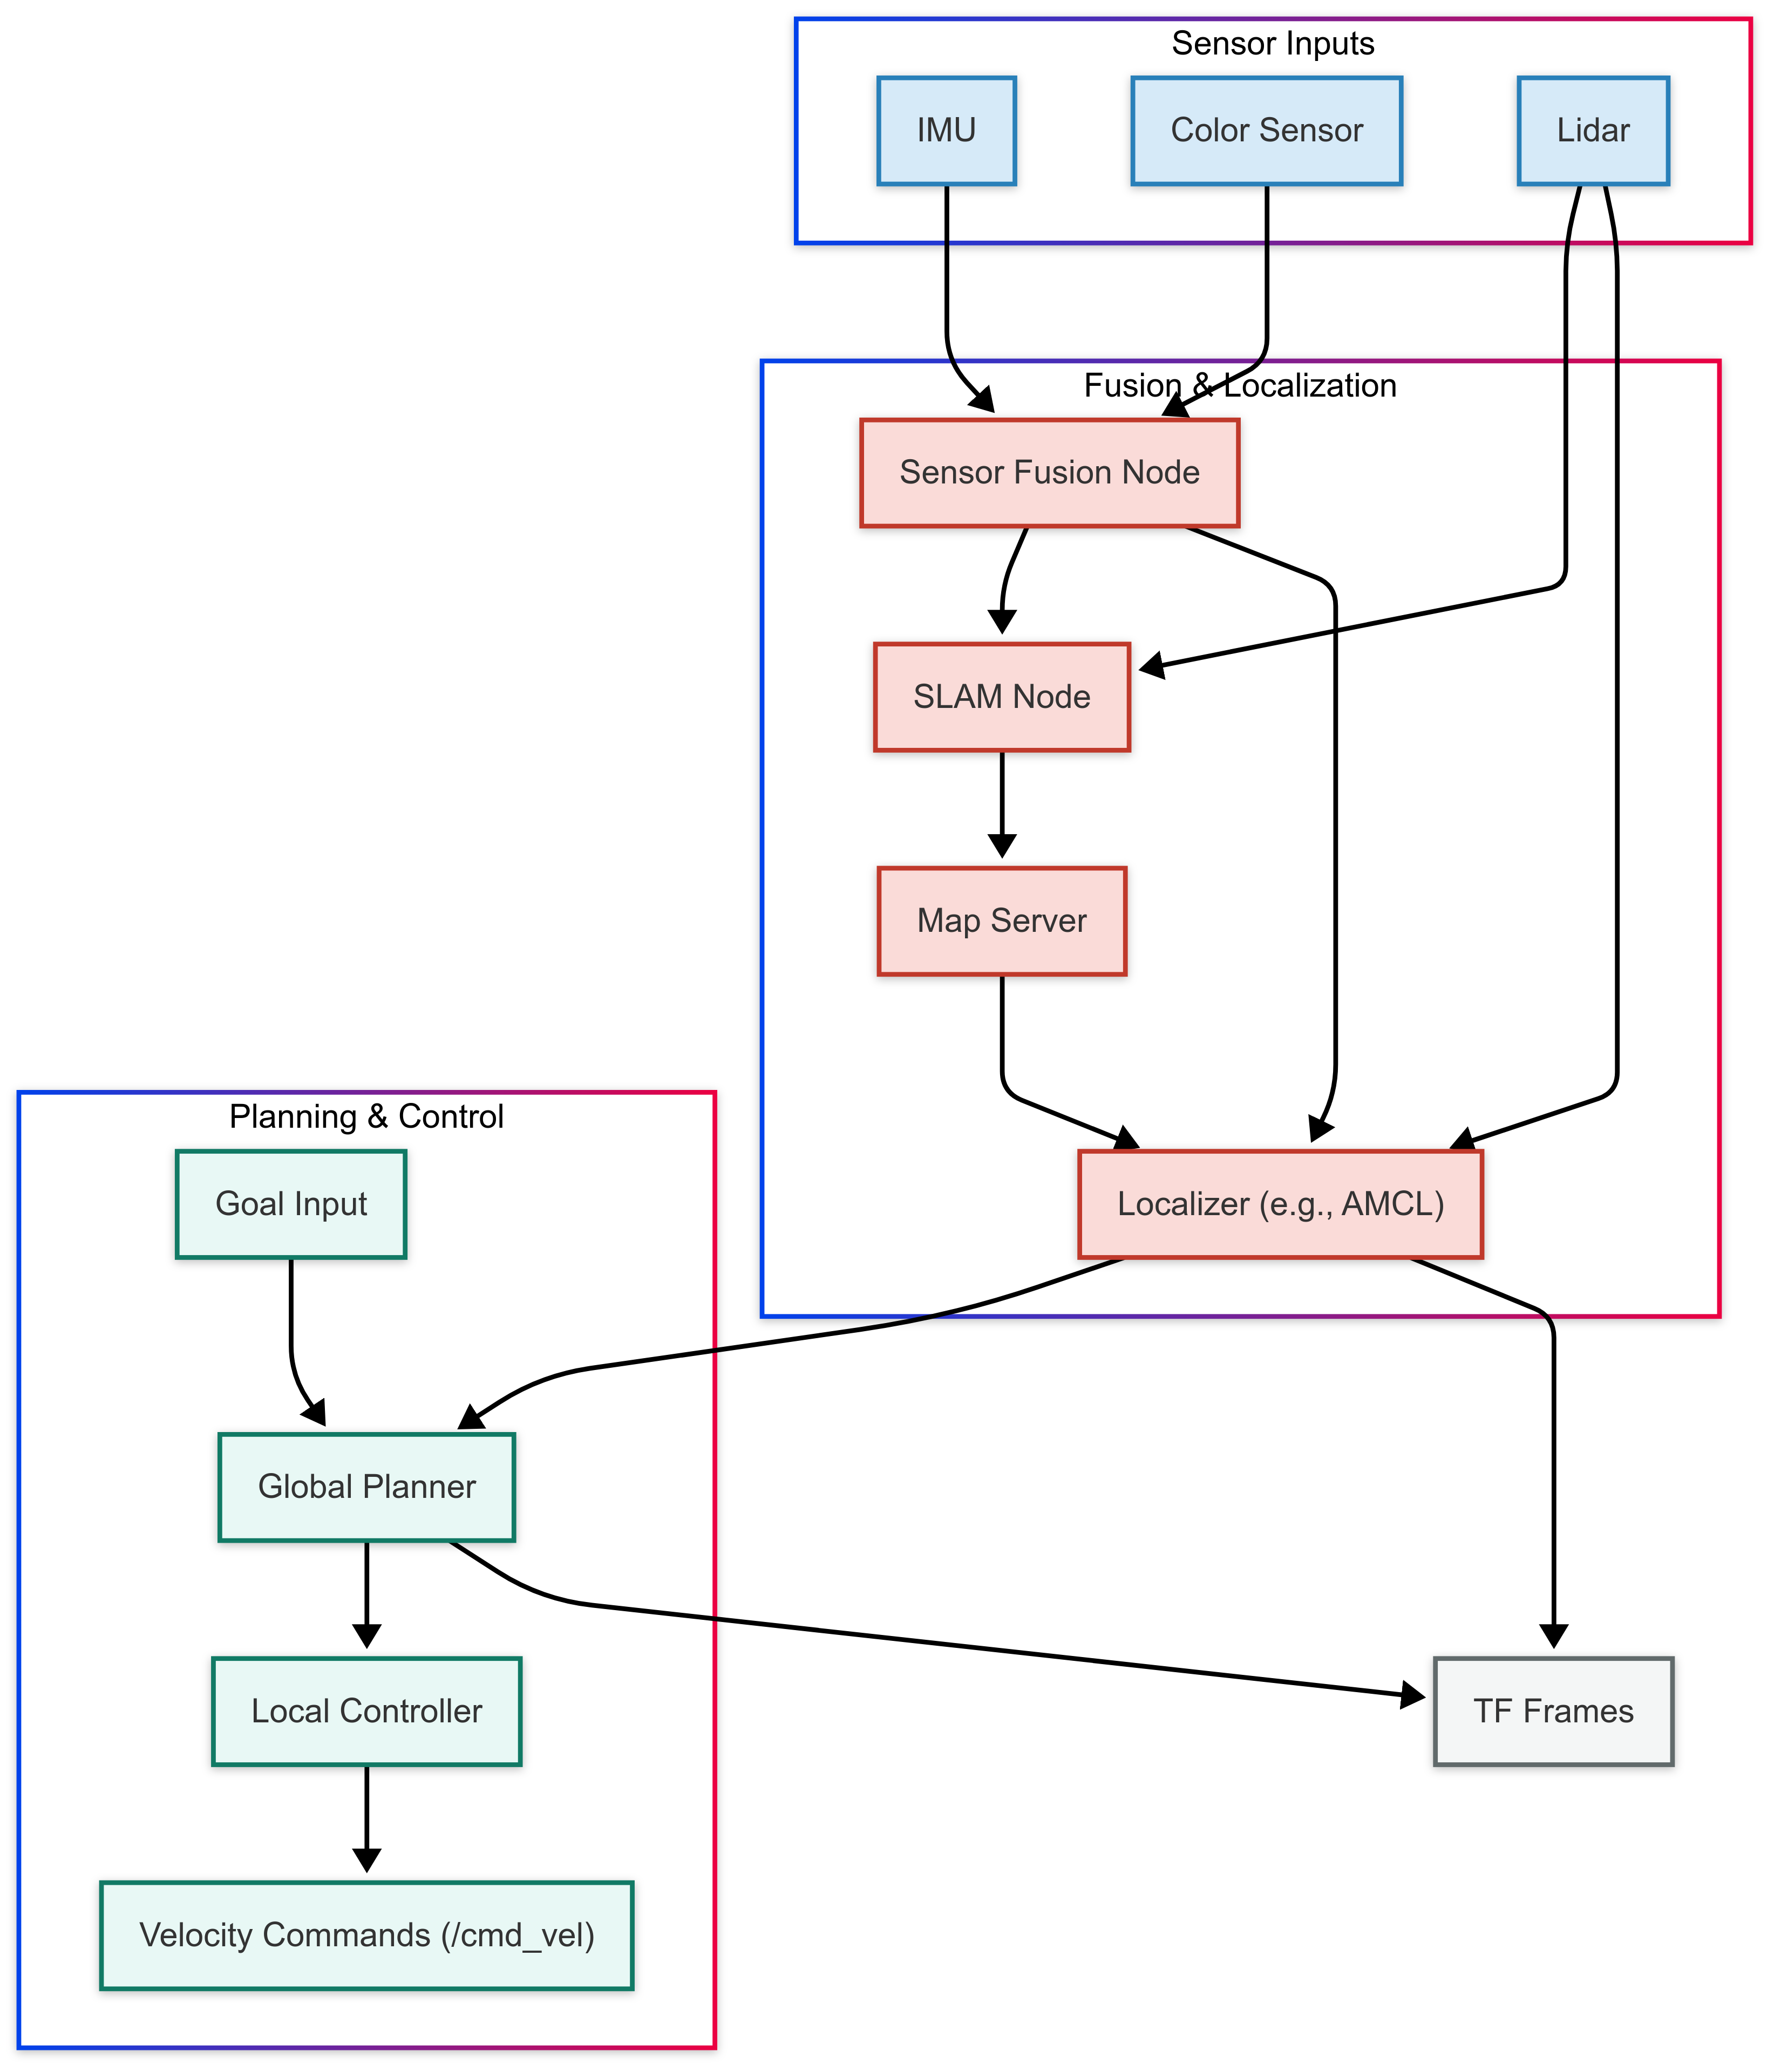
\includegraphics[width=0.7\textwidth]{img/result/Editor _ Mermaid Chart-2025-03-23-223140.png} 
    \caption{ROS 2 navigation pipeline. Sensor inputs are fused to estimate robot odometry. Lidar and fused odometry are used by SLAM and localization modules to estimate position. The navigation stack uses the estimated pose and goal input to generate global plans and local velocity commands for actuation.}

    \label{fig:Nav2 data flow}
\end{figure}
% \subsection{Autonomous Decision-Making}

% A manual control system was implemented to allow basic vehicle movements, but the autonomous decision-making algorithms are still in the development stage. Tests have been initiated to integrate these algorithms, which will allow the system to make real-time decisions based on the environment.



% \subsection{Camera Integration for Object Recognition}

% The integration of the camera with the YOLO object recognition model has shown promising results in controlled environments. However, further testing in real-world conditions is necessary to improve the system's ability to handle different lighting and environmental conditions.

\subsection{Calibration Results}
To ensure accurate sensor measurements and system responses, a comprehensive calibration process was conducted. The key calibration results are summarized below:
\begin{itemize}
    \item LIDAR Calibration: After calibration, distance measurement error was reduced to $\pm 2 \text{cm}$.
    \item IMU Calibration: Bias correction significantly improved orientation estimation.
    \subsubsection{IMU Calibration}
Accurate IMU calibration is essential for improving orientation estimation and reducing sensor drift. The calibration was performed using the Ferraris calibration method, as described in \cite{ferraris_calibration}, with the `imucal` Python library \cite{imucal_docs}.
%https://imucal.readthedocs.io/en/latest/guides/ferraris_guide.html
\paragraph{Calibration Procedure}
The Ferraris calibration process involves collecting IMU measurements while performing controlled multi-axis rotations. This allows for accurate estimation of:
\begin{itemize}
    \item Bias in accelerometer and gyroscope readings.
    \item Scale factor and misalignment corrections.
    \item Soft-iron and hard-iron magnetometer distortions (if applicable).
\end{itemize}

The raw IMU data was logged during the calibration procedure and then processed using `imucal`. The calibration parameters were estimated and applied to the sensor data to correct systematic errors.

\paragraph{Results and Improvements}
After applying the calibration parameters, the following improvements were observed:
\begin{itemize}
    \item Bias drift in the gyroscope was significantly reduced, leading to more stable orientation estimation over time.
    \item Accelerometer readings exhibited improved linearity, ensuring better state estimation in motion.
    \item The overall sensor fusion accuracy improved when integrating the corrected IMU data with other localization sources.
\end{itemize}

Figure~\ref{fig:imu_calibration} illustrates the effects of calibration on IMU measurements, showing the raw data versus corrected data. The improved consistency in sensor readings is evident.

\begin{figure}[h]
    \centering
    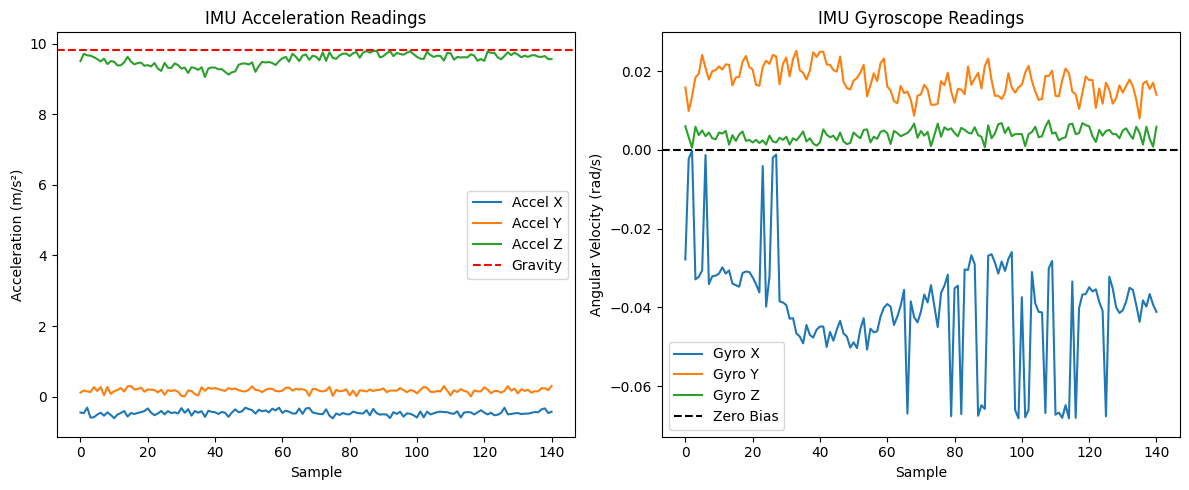
\includegraphics[width=0.8\textwidth]{img/result/imu_before_calib.png}
    \caption{imu\_calibration\_before}
    \label{fig:imu_calibration_before}
\end{figure}

\begin{figure}[h]
    \centering
    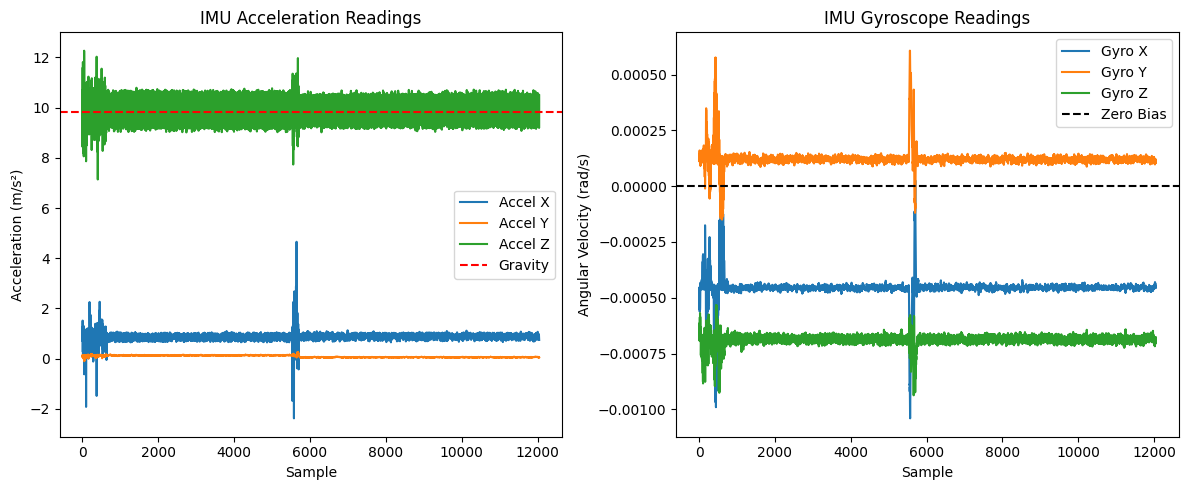
\includegraphics[width=0.8\textwidth]{img/result/imu_after_calib.png}
    \caption{imu\_after\_calib.}
    \label{fig:imu_calibration}
\end{figure}
These calibration steps have significantly enhanced the accuracy of orientation estimation, contributing to improved sensor fusion performance in the overall system.


    \item Odometry Calibration: Encoder-based odometry drift was reduced from 15\% to 5\%.

    %% ask fazil about odom
    
    \item Color Sensor Calibration: Improved accuracy in detecting lane markers under varying lighting conditions.

    % highlight the changes happedn in color sensor 1. width of strips, 2. reduction of speed of vehicles as it was giving out reading in uneven frequency.
    
    \item Motor Controller Calibration: PWM signal tuning optimized motor speed control, improving motion smoothness.
\end{itemize}

\subsection{Challenges and Future Work}

Several challenges remain, particularly with dynamic obstacle avoidance, sensor fusion, and real-time data processing. These areas will be addressed in the next phase of development, where further optimization and real-world testing will be carried out. The integration of real-time feedback and further fine-tuning of the decision-making algorithms are key tasks for the successful deployment of the autonomous vehicle.

\subsection{Summary of Results}

The system has shown significant progress in its ability to perform basic navigation tasks, integrate sensors, and execute basic decision-making algorithms. However, full autonomous operation is still a work in progress. The upcoming tasks focus on refining the autonomous navigation, integrating real-time decision-making, and optimizing the system for real-world deployment.
\end{document}
\documentclass[english,project]{buwthesis}
\begin{document}
\chapter{Conclusion and Future Directions}

\section*{Future Directions}

To enhance the capabilities of the developed robot, the following improvements are proposed. These are categorized based on implementation complexity and priority.

\subsection*{1. Easy / High Priority Enhancements}
\begin{itemize}
    \item Integrate a camera for live video feed and remote monitoring.
    \item Add object detection using pretrained neural networks (e.g., MobileNet, YOLO).
    \item Mount ultrasonic sensors at each corner for blind spot detection.
    \item Improve TF tree by refining static transforms and buffering.
    \item Integrate magnetenometer for steering feedback and also before it check do calibration.
    \item Developing package for Calibration of all sensors
\end{itemize}

\subsection*{2. Mid-Level Enhancements}
\begin{itemize}
    \item Implement a ROS~2-compatible tricycle joint controller for realistic drive behavior.
    \item Add wheel encoders to enhance odometry accuracy.
    \item Incorporate real-time obstacle avoidance using costmaps and local planner adjustments.
    \item Build a real-time monitoring dashboard for sensor and robot state feedback.
\end{itemize}

\subsection*{3. Advanced / Research-Grade Extensions}
\begin{itemize}
    \item Fuse camera, Lidar, and IMU data for robust 3D SLAM.
    \item Experiment with deep learning-based perception and control methods.
    \item Add autonomous goal selection and task-level decision-making modules.
    \item Extend to multi-robot systems with inter-robot coordination.
    \item Optimize deployment for edge devices like NVIDIA Jetson or Google Coral.
\end{itemize}



\end{document}



% Bibliography
\printbibliography[heading=bibintoc]

% Appendix
\appendix
% \chapter{My First Appendix}
% This was just missing.
% \begin{minted}{python}

   
% \end{minted}


\chapter{Implementation of a Color Sensor-Based Steering Angle Measurement System}\label{chap:color_sensor}
\section{Introduction}
In this project, a \textbf{TCS34725 color sensor} was utilized to determine the steering angle based on color stripe detection on a disc attached to the steering shaft.

\section{Initial Approach: Directly Placing the Striped Disc on the Steering Shaft}
Initially, a \textbf{striped disc} was directly mounted on the \textbf{steering shaft}, with the \textbf{TCS34725 color sensor} detecting color transitions as the shaft rotated. The objective was to measure the steering angle.The \textbf{TCS34725 sensor} detects the colored stripes on the disc and determines the direction and magnitude of rotation based on predefined color sequences:
\begin{itemize}
    \item \textbf{Right Turn:} \textbf{RGBRGB} sequence detected.
    \item \textbf{Left Turn:} \textbf{BGRBGR} sequence detected.
\end{itemize}

\subsection{Stripes Used in Direct Disc Approach and Angle Per Stripe Calculation}
To evaluate the effectiveness of different stripe densities (12, 15, and 24 stripes), multiple configurations were tested:
\begin{itemize}
   The steering angle per stripe transition is given by \( \theta = \frac{360^\circ}{N} \), where \( N \) is the number of stripes.


% Insert diagrams here
\begin{figure}[h]
    \centering
    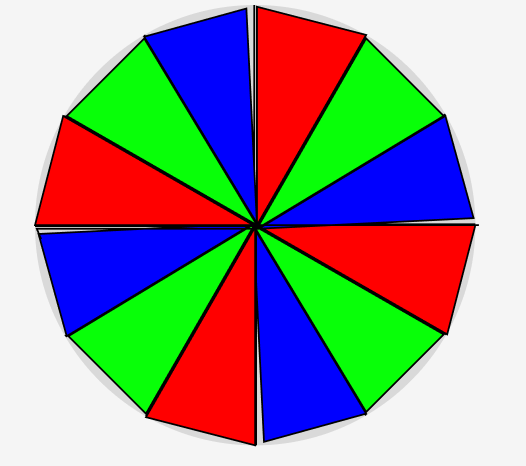
\includegraphics[width=0.3\textwidth]{img/appendix/disc_12_stripes.png}
    \caption{Disc with 12 stripes (6 RGB, 6 BGR).}
    \label{fig:disc_12}
\end{figure}

\begin{figure}[h]
    \centering
    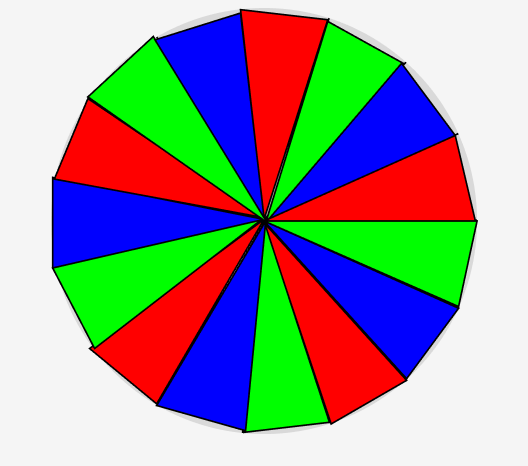
\includegraphics[width=0.3\textwidth]{img/appendix/disc_15_stripes.png}
    \caption{Disc with 15 stripes.}
    \label{fig:disc_15}
\end{figure}

\begin{figure}[h]
    \centering
    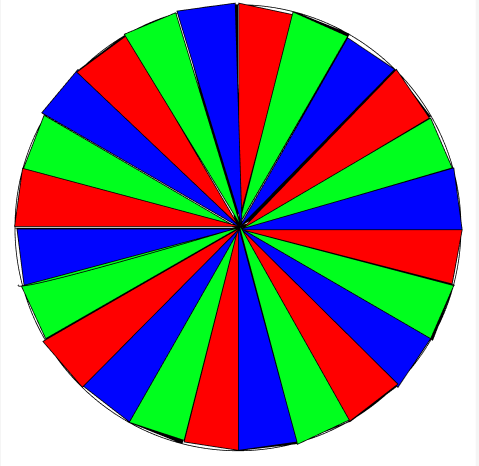
\includegraphics[width=0.3\textwidth]{img/appendix/disc_24_stripes.png}
    \caption{Disc with 24 stripes.}
    \label{fig:disc_24}
\end{figure}


\end{itemize}

\subsection{Limitations of Initial Stripe Detection}
Initially, with 12 stripes (6 RGB, 6 BGR), the system could only determine left or right steering based on the initial color detection. If the sensor started at green, detecting red indicated a left turn, while detecting blue indicated a right turn. However, this approach lacked precise angular resolution, as it only provided binary feedback rather than incremental steering angles.

To improve resolution, tests were conducted with 15 and 24 stripes. However, increasing the stripe count reduced individual stripe width, leading to detection failures. The sensor struggled to differentiate adjacent stripes due to color blending and its limited resolution. This made fine-grained angle measurement unreliable and inconsistent.





\subsection{Solution: Using Lego Gears to Amplify Motion}
To overcome these limitations, a \textbf{gear mechanism} was introduced to \textbf{amplify the rotation} of the steering shaft before transferring it to the striped disc. This \textbf{increased the effective angular displacement}, allowing the sensor to detect stripe transitions more effectively.



\section{Required Calculations}

\subsection{Gear Train Mechanism for Amplification}


The gear ratio is calculated as:
\[
\text{Gear Ratio} = \frac{\text{Driven Gear Teeth}}{\text{Driving Gear Teeth}}
\]

\subsubsection{Gear Ratio 25:1 Configuration }
In this setup, the steering shaft is connected to a 40-tooth input gear, which meshes with an 8-tooth intermediate gear. This intermediate gear shares its shaft with a second intermediate gear, also having 40 teeth. The second intermediate gear is meshed with the final output gear, which has 8 teeth and is mounted on the striped disc. The total gear ratio for this setup is:
\[
\frac{40}{8} \times \frac{40}{8} = 5 \times 5 = 25:1
\]

\subsubsection{Gear Ratio 8.33:1 Configuration (Using 24-Tooth Driven Gear)}

\[
\frac{40}{8} \times \frac{40}{24} = 5 \times 1.67 = 8.33:1
\]


\subsection{Strip Spacing Calculation in Gear Mechanism}
With the gear train, the disc’s full \( 360^\circ \) rotation was mapped to the amplified steering motion. The steering angle per stripe transition is calculated using the general formula:

\[
\theta_{\text{steering}} = \frac{360^\circ}{N} \times \frac{1}{\text{Gear Ratio}}
\]

where \( N \) is the number of stripes on the disc, and the gear ratio determines the amplification factor. This formula demonstrates how increasing stripe count and applying different gear ratios influence the final steering movement per detected transition.


\begin{table}[h]
    \centering
    \caption{Strip Spacing Calculation for Different Gear Ratios}
    \begin{tabular}{lccc}
        \toprule
        Stripes & Transition per Stripe (\(^\circ\)) & Steering Angle After 25:1 (\(^\circ\)) & Steering Angle After 8.33:1 (\(^\circ\)) \\
        \midrule
        12      & 30\(^\circ\)                      & 1.2\(^\circ\)                         & 3.6\(^\circ\)                         \\
        15      & 24\(^\circ\)                      & 0.96\(^\circ\)                        & 2.88\(^\circ\)                        \\
        24      & 15\(^\circ\)                      & 0.6\(^\circ\)                         & 1.8\(^\circ\)                         \\
        \bottomrule
    \end{tabular}
\end{table}



\subsection{Challenges and Difficulties Faced}
Despite implementing the gear mechanism to amplify the rotation and improve stripe detection, several challenges persisted:
\begin{itemize}
    \item \textbf{Disc Stability Issues:}
    \begin{itemize}
        \item If the disc which is made of cardboard sheet was tightly connected to the driven shaft, it experienced excessive \textbf{recoil after the gear stopped rotating}, causing unintended stripe transitions.
        \item If the disc was not connected tightly, it \textbf{did not rotate as much as expected}, leading to incorrect tick counts and inconsistent steering angle readings.
    
        \item \textbf{Weight Considerations:} When a printed disc was used for more durability, it was \textbf{too heavy for the Lego gears}, leading to additional instability and erratic movement.
    \end{itemize}
   
    \item \textbf{Precision Issues in Color Sensing:}
    \begin{itemize}
        \item The \textbf{TCS34725 sensor} had a \textbf{small sensing area}, requiring the \textbf{stripes to be perfectly aligned} for accurate detection.
        \item Variations in lighting conditions and sensor positioning also \textbf{caused fluctuations in color readings}, leading to occasional false detections.
    \end{itemize}
    
\end{itemize}


\section{Conclusion: Transition to a Magnetic Sensor}
Due to \textbf{significant stability challenges} with the color-coded disc system, a decision was made to transition to a \textbf{magnetic sensor (AS5600)} for measuring steering angles. Assuming that the magnetic sensor provides higher accuracy without reliance on visual transitions, better durability unaffected by mechanical instability, and simpler integration without the need for extensive gear train modifications.



\end{document}

